%!TEX root = tzplot-doc.tex
%\begin{document}

%%%==========================
\part{Points, Lines, and Curves}
%%%==========================
\label{p:linesandcurves}


%%==================================
\chapter{Getting Ready}
\label{c:gettingready}

%%------------------------------------------------------------
\section{Styles: \texttt{tzdotted}, \texttt{tzdashed}, \texttt{tzhelplines}}
\label{s:styles:tzhelplines}

The styles \ixttw{tzdotted}, \ixttw{tzdashed}, and \ixttw{tzhelplines} are defined as follows:

\begin{tzsty}{}
% styles: tzdotted, tzdashed, tzhelplines
\tikzset{%
  tzdotted/.style={line cap=round,dash pattern=on 0pt off 1cm/(#1)},
  tzdotted/.default=10
}
\tikzset{%
  tzdashed/.style={dashed=none,dash pattern=on 5mm/(#1) off 5mm/(#1)},
  tzdashed/.default=10
}
\tikzset{%
  tzhelplines/.style={help lines,-,tzdotted}
}
\end{tzsty}

The styles |tzdotted| and |tzdashed| print 10 dots and 10 dashes per 1cm, respectively, by default.
The style |tzhelplines| uses |tzdotted| by default.


%%------------------------------------------------------------
\section{\protect\cmd{\tzhelplines}, \protect\cmd{\tzhelplines*}}
\label{s:tzhelplines}

\icmd{\tzhelplines} draws |grid| from the first coordinate to the second coordinate.
If only one coordinate is specified, then the first coordinate is regarded as |(0,0)|.

The starred version \icmd{\tzhelplines*} uses the grid as a \iisw{bounding box}.

\begin{tzdef}{}
% syntax: minimum
\tzhelplines(<coor>)
% syntax: full
\tzhelplines[<opt>](<coor1>)(<coor2>)
% defaults
  [help lines,tzdotted=10](<m>)()
% (<m>): mandatory argument
\end{tzdef}

Here, |(|\ixxw{<m>}|)| stands for a \xem{mandatory} argument.

\begin{tztikz}{}
\tzhelplines(4,3)      % works similarly to:
  \draw [help lines] (0,0) grid (4,3);

\tzhelplines(1,1)(4,3) % works similarly to:
  \draw [help lines] (1,1) grid (4,3);
\end{tztikz}


By default, |\tzhelplines| prints |grid| with |10| dots per |1cm|.
|\tzhelplines| with the option value |[tzdotted=<n>]| prints |<n>| dots per |1cm|.
(That is, the default value is |tzdotted=10|.)

\begin{tzcode}{.3}
% \tzhelplines
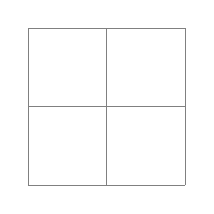
\begin{tikzpicture}
\tzhelplines(2,2)
\draw [help lines] (3,0) grid (5,2);
\end{tikzpicture}
\end{tzcode}


\begin{tzcode}{.3}
% tzdotted: (default: 10 dots per 1cm)
\begin{tikzpicture}
\tzhelplines[thick](1,2)                  % 10 dots
\tzhelplines[thick,tzdotted=20](2,0)(3,2) % 20 dots
\tzhelplines[thick,tzdotted=5](4,0)(5,2)  %  5 dots
\end{tikzpicture}
\end{tzcode}

With the option value, |[tzdotted=<n>/<d>]|, |\tzhelplines| prints |<n>| dots per |<d>cm|.

Similarly for |tzdashed|.

\begin{tzcode}{.3}
% tzdotted, tzdashed
\begin{tikzpicture}
\tzhelplines[thick,tzdashed](4,2)
\tzhelplines[thick,step=.5](4,2)
\end{tikzpicture}
\end{tzcode}

\begin{tzcode}{.3}
% scaled: 7 dots per .7cm (10 dots per hard 1cm)
\begin{tikzpicture}[scale=.7]
\tzhelplines[tzdashed](4,3)
\tzhelplines[step=.5](4,3)
\end{tikzpicture}
\end{tzcode}

\begin{tzcode}{.3}
% scaled: 10/.7 means 10 dots per .7cm
\begin{tikzpicture}[scale=.7]
\tzhelplines[tzdashed=10/.7](4,3)         %%
\tzhelplines[step=.5,tzdotted=10/.7](4,3) %%
\end{tikzpicture}
\end{tzcode}


%%------------------------------------------------------------
\section{\protect\cmd{\tzbbox}: A bounding box}
\label{s:tzbbox}

\icmd{\tzbbox} sets a bounding box.

\begin{tzdef}{}
% syntax
\tzbbox(<coor1>)(<coor2>)
% defaults
  (0,0)(<m>)
\end{tzdef}

\begin{tztikz}{}
\tzbbox(-1,-1)(4,3) % is an abbreviation of:
  \path [ use as bounding box ] (-1,-1) rectangle (4,3);
\end{tztikz}

If only one coordinate is specified, the first coordinate is regarded as |(0,0)|.

%%==================================
\chapter{Dots}
\label{c:dots}

%%------------------------------------------------------------
\section{\protect\cmd{\tzcdot(*)}: A small circle}
\label{s:tzcdot}

A dot is usually expressed by a small circle.
\icmd{\tzcdot} prints a circle dot \tikz \tzcdot(0,0);.

The starred version \icmd{\tzcdot*} prints a filled circle dot \tikz \tzcdot*(0,0);.
The \xem{radius} of the circle is |1.2pt|, by default.

\begin{tzdef}{}
% syntax: minimum
\tzcdot(<coor>)
% syntax: medium
\tzcdot*(<coor>){<label>}[<angle>](<radius>)
% syntax: full
\tzcdot*[<opt>]<shift coor>(<coor>){<label>}[<[label opt]angle>](<radius>)
% defaults
 *[ solid,thin,tzcdot=1.2pt ]<>(<m>){}[](1.2pt)
% tzcdot is a predefined key (in this package).
% (<m>): mandatory
\end{tzdef}

Here, |(|\ixxw{<m>}|)| stands for a \xem{mandatory} argument. All others are optional arguments.

\paragraph{How to change the size}
There are three ways to change the \xem{radius} of a circle dot drawn by |\tzcdot|.

\begin{enumerate}
\item The simplest way is to use the last parenthesis option, like |\tzcdot(0,0)(3pt)|.

\begin{tztikz}{}
\tzcdot(0,0)       % is an abbreviation of:
  \draw (0,0) circle (1.2pt); % default radius=1.2pt
\end{tztikz}

\begin{tztikz}{}
\tzcdot*(0,0)(3pt) % is an abbreviation of:
  \draw [fill] (0,0) circle (3pt);
\end{tztikz}

\item
You can use the key-value option |[tzcdot=<dim>]|, like |\tzcdot[tzcdot=3pt](0,0)|,  to change the \xem{radius} of a circle dot. The |tzcdot| key is defined in the package.
If both the |tzcdot| key-value and the last parenthesis option are used, the former wins.

\begin{tztikz}{}
\tzcdot*(1,1) % works like:
  \draw [fill] (1,1) circle [radius=1.2pt]; % default radius=1.2pt
\end{tztikz}

\begin{tztikz}{}
\tzcdot*[tzcdot=3pt] % works like:
  \draw [fill] (0,0) circle [radius=3pt];
\end{tztikz}

\begin{tzcode}{.3}
% \tzcdot(*)
\begin{tikzpicture}
\tzhelplines(4,2)
\tzcdot(0,0)        \tzcdot[tzcdot=4pt](1,1)
\tzcdot*(2,1)(2pt)  \tzcdot*(3,0)(3pt)
\end{tikzpicture}
\end{tzcode}

\item 
Another way to change the radius is to use a macro, like |\settzcdotradius{3pt}|,
It is effective within the |tizpicture| environment unless changed by \icmd{\settzcdotradius} again.

\begin{tzcode}{.3}
% \settzcdotradius
\begin{tikzpicture}
\tzhelplines(4,2)
\settzcdotradius{4pt}
\tzcdot(0,0)        \tzcdot(1,1)
\tzcdot*(2,1)(2pt)  \tzcdot*(3,0)
\end{tikzpicture}
\end{tzcode}

\end{enumerate}


\paragraph{How to label}
You can add a label to a specified coordinate by adding the optional argument |{<label>}| immediately after |(<coor>)|. You can also change the |<label>| position by the option |[<angle>]|.
(Note that you \xem{cannot} use the abbreviations such as |a|, |r|, |bl|, etc. to place label nodes.)

\begin{tztikz}{}
\tzcdot(0,0){A} % is an abbreviation of:
  \draw (0,0) circle (1.2pt) node [label={:A}] {};

\tzcdot(0,0)(2pt){A}[[blue]0] % is an abbreviation of:
  \draw (0,0) circle (2pt) node [label={[blue]0:A}] {};
\end{tztikz}

\begin{tzcode}{.3}
% \tzcdot: labels
\begin{tikzpicture}
\tzhelplines(4,3)
\tzcdot(0,0){A} % default position: 90 or above
\tzcdot[tzcdot=4pt](1,1){B}[0]
\tzcdot*(2,1){C}[45](2pt)
\tzcdot*(3,0){D}[-90](3pt)
\tzcdot(4,3){E}[-90](6pt)
\end{tikzpicture}
\end{tzcode}

The label position does not depend on the size of circle dots.

\paragraph{How to change colors}
With the first optional argument |[<opt>]|, you can change the color of a dot.
You can also change the color of a label, as shown in the following example.

\begin{tzcode}{.3}
% \tzcdot(*)

\begin{tikzpicture}
\draw [help lines] (0,0) grid (4,3);
\tzcdot(0,0){A}
\tzcdot*[red](1,0){\textbf{B}}[45]
\tzcdot*[red,fill=green](2,1){green}[[blue]0](10pt)
\tzcdot[tzcdot=2*7pt](3,2){big}[center]
\tzcdot*[fill=red,text=blue](4,3){D}(2*3pt)
\end{tikzpicture}
\end{tzcode}


\paragraph{Shift}
Dots can be shifted by specifying the optional argument |<shift coor>| immediately before |(<coor>)|. The empty shift option |<>| is not allowed.

\begin{tzcode}{.3}
% \tzcdot: shift

\begin{tikzpicture}
\draw [help lines] (0,0) grid (4,3);
\tzcdot(0,0){A}
\tzcdot*[red]<0,2>(1,0){\textbf{B}}[45] % shift
\tzcdot*[red,fill=green](2,1){green}[[blue]0](10pt)
\tzcdot[tzcdot=2*7pt]<1,-1>(3,2){big}[center] % shift
\tzcdot*[fill=red,text=blue](4,3){D}(2*3pt)
\end{tikzpicture}
\end{tzcode}

\begin{tzcode}{.3}
% \tzcdot: repeated
\begin{tikzpicture}
\tzhelplines(4,2)
\foreach \x in {0,...,4}
  { \foreach \A in {2,4,6,8}
      { \tzcdot[blue]    (\x,0)(\A pt) } }
\foreach \x in {0,...,4}
  { \foreach \A in {2,4,6,8}
      { \tzcdot[red]<1,1>(\x,0)(\A pt) } } % shift
\end{tikzpicture}
\end{tzcode}


%%------------------------------------------------------------
\section{\protect\cmd{\tzcdots(*)}: Multiple circle dots}
\label{s:tzcdots}

The macro \icmd{\tzcdots} takes an arbitrary number of coordinates as arguments to print multiple circle dots with the radius |1.2pt|, by default.
You need to indicate when the iteration of an arbitrary number of coordinates ends, by typing a \xem{semicolon} |;|.
Let us call this kind of macro a \iisw{semicolon version} macro.

\remark
\begin{itemize}
\item DO NOT FORGET to enter `|;|' at the end of iteration.
  \begin{itemize}
  \item Tokens such as `|!|' and `|#|' other than the open parenthesis `|(|' work like the semicolon `|;|' to indicate the end of iteration.
        But it is highly recommended to use `|;|' for consistency.
  \end{itemize}
\item Without the semicolon |;|, the macro does nothing or a compile error occurs.
\end{itemize}


The starred version |\tzcdots*| prints multiple filled dots.

\begin{tzdef}{}
% syntax: minimum
\tzcdots*(<coor>)(<coor>)..repeated..(<coor>) ;
% syntax: full
\tzcdots*[<opt>]<shift coor> (<coor>){<label>}[<[label opt]angle>]
                            ..repeated.. (){}[] ; (<dot radius>)
% defaults
 *[tzcdot=1.2pt]<>(<m>){}[]..repeated..(){}[] ; (1.2pt)
\end{tzdef}

\begin{tzcode}{.3}
% \tzcdots(*)
\begin{tikzpicture}
\tzhelplines(4,3)
\tzcdots(0,0)(1,1)(2,1)(3,2)(4,0);
\tzcdots*(0,3)(1,2)(2,2)(3,3)(4,3);
\end{tikzpicture}
\end{tzcode}

\paragraph{How to label}

Each coordinate can be followed by the optional arguments |{<label>}| and |[<angle>]| to label dots. So the repeating pattern is the triple |(<coor>){<label>}[<angle>]|.

\begin{tzcode}{.3}
% \tzcdots: label
\begin{tikzpicture}
\tzhelplines(4,3)
\tzcdots(0,0){A}
        (1,1)
        (2,1){C}[0]
        (3,2){D}[-90]
        (4,0){E};
\tzcdots*(0,3)(1,2){B}(2,2){C}[45](3,3)(4,3);
\end{tikzpicture}
\end{tzcode}

\paragraph{How to change the size of dots}

There are three ways of changing the \xem{radius} of dots.
\begin{enumerate}
\item The simplest way is to use the \xem{last} parenthesis optional argument, \xem{after the semicolon}.
\item Another way is to use the \ixxw{tzcdot} key, like |\tzcdots[tzcdot=3pt]...|.
If both options are used the key-value option wins.
\item You can also use the macro \icmd{\settzcdotradius}.
The effect remains within the |tikzpicture| environment unless it is changed again.
\end{enumerate}

\begin{tzcode}{.3}
% \tzcdots: size (radius)
\begin{tikzpicture}
\tzhelplines(4,3)
\settzcdotradius{3pt}
\tzcdots(0,0)(1,0){3pt};
\tzcdots*(1,1)(2,1){1pt};(1pt) % simplest
\tzcdots[tzcdot=5pt](2,2)(3,2){5pt};
\tzcdots*(3,3)(4,3){3pt};
\end{tikzpicture}
\end{tzcode}



\paragraph{How to change colors}

With the first optional argument |[<opt>]|, you can change the color of dots.
You can also change the color of all labels at once using the first optional argument, 
like |\tzcdots[text=red]...| as shown in the following example.

\begin{tzcode}{.3}
% \tzcdots: color
\begin{tikzpicture}
\tzhelplines(4,3)
\settzcdotradius{3pt}
\tzcdots*[red]
  (0,0)(1,1){\textbf{Ben}}[[blue]-90](2,1)(3,0);
\tzcdots*[thick,blue,fill=green,text=red]
  (1,2){A}(2,2){Ben}[[blue]-90](3,2){C}(4,2){D};(4pt)
\tzcdots*[blue]
  (1,3){A}(2,3){B}(3,3){C}(4,3){D};
\end{tikzpicture}
\end{tzcode}

\paragraph{Shift} You can move the coordinates of dots by specifying |<shift coor>| option immediately before the first coordinate.

\begin{tzcode}{.3}
% \tzcdots: shift
\begin{tikzpicture}
\tzhelplines(4,3)
\tzcdots[red] (0,0){A}(1,1)(2,1){C}(3,2){D}[0](4,0){E};
\tzcdots*<0,1>(0,0){A}(1,1)(2,1){C}(3,2){D}[0](4,0){E};
\end{tikzpicture}
\end{tzcode}


%%------------------------------------------------------------
\section{\protect\cmd{\tzdot(*)}: A single node dot}
\label{s:tzdot}

The macro \icmd{\tzdot} prints a small circle node \tikz \tzdot(0,0);, as a dot, with the \xem{diameter} (or |minimum size|) of |2.4pt|, by default.

The starred version \icmd{\tzdot*} prints a filled dot \tikz \tzdot*(0,0);.

\begin{tzdef}{}
% syntax: minimum
\tzdot(coor)
% syntax: medium
\tzdot*(<coor>){<label>}[<angle>](<dot size>)
% syntax: full
\tzdot*[<node opt>]<shift coor>(<coor>){<label>}[<[label opt]angle>](<dot size>)
% defaults
 *[ tzdot=2.4pt ]<>(<m>){}[](2.4pt)
% the style tzdot is predefined
% (<m>): mandatory
\end{tzdef}

|\tzdot(*)| accepts one mandatory argument, denoted by |(|\ixxw{<m>}|)|. All others are optional.

The style \ixxw{tzdot} is defined as follows:

\begin{tzsty}{}
% style: tzdot
\tikzset{
  tzdot/.style={draw,circle,solid,thin,inner sep=0pt,minimum size=#1},
  tzdot/.default=2.4pt
}
\end{tzsty}


\subsection{{\normalfont\scshape Three Ways} to change the size of node dots}
\label{ss:threeways}

There are \iscw{Three Ways} to change the \xem{diameter} (or |minimum size|) of a node dot drawn by |\tzdot(*)|.

\begin{enumerate}
\item Use the predefined style |tzdot| in the first optional agrument, like |\tzdot[tzdot=5pt](0,0)|, which gives the same result as |\tzdot[minimum size=5pt](0,0)|.

\begin{tztikz}{}
\tzdot(0,0) % works like:
  \path (0,0) node [tzdot=2.4pt] {}; % default size
  % or equivalently
  \node [tzdot,minimum size=2.4pt] at (0,0) {};
\end{tztikz}

\item The simplest way is to use the \xem{last} parenthesis optional argument, like |\tzdot(0,0)(5pt)|, which yields the same result as in |\tzdot[tzdot=5pt](0,0)|.
If both options are used, the |tzdot| (or |minimum size|) option overwrites the last parenthesis option.

\begin{tzcode}{.3}
% \tzdot(*)
\begin{tikzpicture}
\tzhelplines(4,2)
\tzdot(0,0)        \tzdot[tzdot=8pt](1,1)
\tzdot*(2,1)(4pt)  \tzdot*(3,0)(6pt)
\end{tikzpicture}
\end{tzcode}

\item To change the size of all node dots drawn by |\tzdot*|, you can use the macro |\settzdotsize|. Its effect remains valid until the end of |tikzpicture| environment unless changed again.

\begin{tzcode}{.3}
% \settzdotsize
\begin{tikzpicture}
\tzhelplines(4,2)
\settzdotsize{8pt}
\tzdot(0,0)        \tzdot(1,1)
\tzdot*(2,1)(4pt)  \tzdot*(3,0)
\end{tikzpicture}
\end{tzcode}

\end{enumerate}

\subsection{How to label}
\label{ss:tzdot:label}

You can add a label to a specified coordinate by specifying the optional argument |{<label>}| immediately after the coordinate |(<coor>)|.

You can also change the label position by the option |[<angle>]| following |{<label>}|.

\begin{tztikz}{}
\tzdot(0,0){A}(3pt)          % works like:
  \path (0,0) node [tzdot=3pt,label={:A}] {};
  
\tzdot*(0,0){A}[[red]0](3pt) % works like:
  \path (0,0) node [fill,tzdot=3pt,label={[red]0:A}] {};
\end{tztikz}


\begin{tzcode}{.3}
% \tzdot: labels
\begin{tikzpicture}
\tzhelplines(4,3)
\tzdot(0,0){A}
\tzdot(1,1){B}[0](8pt)
\tzdot*(2,1){C}[45](4pt)
\tzdot*(3,0){D}[-90](6pt)
\tzdot(4,3){E}[-90](12pt)
\end{tikzpicture}
\end{tzcode}

Unlike |\tzcdot|, the |\tzdot|'s label position depends on the size of a circle node. In \Tikz\ jargon, |{<label>}| is in a \iisw{label node} for a \iisw{main node} that is a circle node with no text in it, so |<label>| moves accordingly as the main node dot gets bigger or smaller.


\subsection{How to change colors and shapes}
\label{ss:tzdot:color}

With the first optional argument |[<node opt>]|, you can change of the color or shape of dots.
You can also change the label color using |[<label opt>]| as shown in the following example.

\remark
\begin{itemize}
\item |[<node opt>]| is for options of \xem{main nodes}, |[<label opt>]| is for options of \xem{label nodes}.
\item |[<label opt>]| is used in the form of |[<[label opt]angle>]|.
\end{itemize}

\begin{tzcode}{.3}
% \tzdot: color

\begin{tikzpicture}
\draw [help lines] (0,0) grid (4,3);
\tzdot(0,0){A}
\tzdot*[red](1,0){\textbf{B}}[45]
\tzdot*[red,fill=green](2,1){green}[[blue]0](2*10pt)
\tzdot[tzdot=4*7pt](3,2){big}[center]
\tzdot*[fill=red](4,3){D}(4*3pt)
\end{tikzpicture}
\end{tzcode}


\begin{tzcode}{.3}
% \tzdot: shape

\begin{tikzpicture}
\draw [help lines] (0,0) grid (4,3);
\tzdot[regular polygon](0,0){A}(10pt)
\tzdot*[red](1,0){\textbf{B}}[45]
\tzdot*[red,fill=green,rectangle](2,1){green}[0](2*10pt)
\tzdot[tzdot=4*7pt](3,2){big}[center]
\tzdot*[fill=red,star](4,3){D}(4*3pt)
\end{tikzpicture}
\end{tzcode}



\subsection{How to move: \texttt{shift}}
\label{ss:tzdot:shift}

Dots can be shifted by specifying the optional argument |<shift coor>| immediately before |(<coor>)|. The empty shift option |<>| is not allowed.

\begin{tzcode}{.3}
% \tzdot: shift

\begin{tikzpicture}
\draw [help lines] (0,0) grid (4,3);
\tzdot[regular polygon](0,0){A}(10pt)
\tzdot*[red]<0,2>(1,0){\textbf{B}-shifted}[45] % shift
\tzdot*[red,fill=green,rectangle](2,1){green}[0](2*10pt)
\tzdot[tzdot=4*7pt]<1,-1>(3,2){big}[center]    % shift
\tzdot*[fill=red,star](4,3){D}(4*3pt)
\end{tikzpicture}
\end{tzcode}


\begin{tzcode}{.3}
% \tzdot: repeated
\begin{tikzpicture}
\tzhelplines(4,2)
\foreach \x in {0,...,4}
  { \foreach \A in {1,2,3,4}
      { \tzdot[blue]      (\x,0)(2*\A mm) } }
\foreach \x in {0,...,4}
  { \foreach \A in {1,2,3,4}
      { \tzdot[green]<1,1>(\x,0)(2*\A mm) } }  % shift
\end{tikzpicture}
\end{tzcode}


\subsection{Comparison: \protect\cmd{\tzdot} and \protect\cmd{\tzcdot}}
\label{ss:tzdot:comparison}

The most important difference between |\tzcdot| and |\tzdot| is that |\tzcdot| is affected by \Tikz's scaling factor, but |\tzdot| is not.
This is critical when |xscale| is not equal to |yscale|.

\begin{tzcode}{.3}
\begin{tikzpicture}[xscale=1.6,yscale=.8]
\tzhelplines(3,3)
\tzcdot(0,0)(3pt)              % dostorted
\tzdot(1,0)(6pt)
\tzcdots*(1,1)(2,1)(3,1);(2pt) % distorted
\tzdots*(1,2)(2,2)(3,2);(4pt)
\end{tikzpicture}
\end{tzcode}

The following table further shows the differences between them.
%Everything else is the same for end-users.

\begin{tzcode}[listing only,colback=green!10!white]{.3}
% concept       % single  % multi    % size control     % [key=default size]
node [circle]   \tzdot    \tzdots    \settzdotsize      [tzdot=2.4pt]  % diameter
circle          \tzcdot   \tzcdots   \settzcdotradius   [tzcdot=1.2pt] % radius
\end{tzcode}

\remark 
\begin{itemize}
\item In \Tikz, a `node' is `not' affected by `scaling' unless the \Tikz\ option |transform shape| is used together.
|\tzdot| is also useful for labelling a large dot.
  \begin{itemize}
  \item In |\tzdot|, |<label>| is a label in a \iisw{label node} for a node dot (as a \iisw{main node}).
  So if a main node dot gets larger or smaller, its label moves accordingly. 
  (Unlike, the labels with |\tzcdot| or |\tzcdots|.)
  \item The position of |<label>| in |\tzcdot| does not depend on the size of dots.
  \end{itemize}
\item The package |tzplot| takes |\tzdot| as a \xem{standard dot}, not |\tzcdot|.
So, you can apply the \threeways\ (on page \pageref{ss:threeways}) to change the size of any standard dots.
\end{itemize}


%%------------------------------------------------------------
\section{\protect\cmd{\tzdots(*)}: Multiple node dots}
\label{s:tzdots}

\icmd{\tzdots} takes an arbitrary number of coordinates as arguments to print multiple circle node dots with the \xem{diameter} (or |minimum size|) of |2.4pt|, by default.

This is a \iisw{semicolon version} macro, with the repeating pattern |(<coor>){<label>}[<angle>]|, which means that you need to type a \xem{semicolon} `|;|' at the end of the coordinate repetition. The \xem{semicolon} says, ``\xem{The repetition ends here}."

\remark
\begin{itemize}
\item DO NOT FORGET to enter `|;|' at the end of iteration.
  \begin{itemize}
  \item Tokens such as `|!|' and `|#|' other than the open parenthesis `|(|' work like the semicolon `|;|' to indicate the end of iteration.
        But it is highly recommended to use `|;|' for consistency.
  \end{itemize}
\item Without the semicolon |;|, the macro does nothing or a compile error occurs.
\end{itemize}

The starred version \icmd{\tzdots*} prints multiple filled node dots.

\begin{tzdef}{}
% syntax: minimum
\tzdots*(<coor>)(<coor>)..repeated..(<coor>) ;
% syntax: full
\tzdots*[<node opt>]<shift coor> (<coor>){<label>}[<[label opt]angle>]
                                 ..repeated.. (){}[] ; (<dot size>)
% defaults
 *[tzdot=2.4pt]<> (<m>){}[] ..repeated.. (){}[] ; (2.4pt)
\end{tzdef}

\begin{tzcode}{.3}
% \tzdots(*)
\begin{tikzpicture}
\tzhelplines(4,3)
\tzdots(0,0)(1,1)(2,1)(3,2)(4,0);
\tzdots*(0,3)(1,2)(2,2)(3,3)(4,3);
\end{tikzpicture}
\end{tzcode}

\paragraph{How to label}

Each coordinate can be followed by the optional arguments |{<label>}| and |[<angle>]| to label dots. So the triple |(<coor>){<label>}[<angle>]| is the whole repeating pattern.

\begin{tzcode}{.3}
% \tzdots: label
\begin{tikzpicture}
\tzhelplines(4,3)
\tzdots(0,0){A}
       (1,1)
       (2,1){C}[0]
       (3,2){D}[-90]
       (4,0){E};
\tzdots*(0,3)(1,2){B}(2,2){C}[45](3,3)(4,3);
\end{tikzpicture}
\end{tzcode}


\paragraph{How to change the size of dots}

There are \threeways\ of changing the \xem{diameter} of node dots, as discussed in Section \ref{ss:threeways} on page \pageref{ss:threeways}.

\begin{enumerate}
\item The simplest way is to use the \xem{last} parenthesis optional argument, \xem{after the semicolon}.
\item Another way is to use the style \ixxw{tzdot}, like |\tzdots[tzdot=3pt]...|.
If both options are used the |tzdot| option style wins.
\item You can also use the macro \icmd{\settzdotsize}.
The effect remains within the |tikzpicture| environment unless it is changed again.
\end{enumerate}

\begin{tzcode}{.3}
% \tzdots: size (diameter)
\begin{tikzpicture}
\tzhelplines(4,3)
\settzdotsize{3mm}
\tzdots(0,0)(1,0){3mm};
\tzdots*(1,1)(2,1){2mm};(2mm) % simplest
\tzdots[tzdot=4mm](2,2)(3,2){4mm};
\tzdots*(3,3)(4,3){3mm};
\end{tikzpicture}
\end{tzcode}



\paragraph{How to change colors}

With the first optional argument |[<node opt>]| you can change the color of node dots.
You can also change the color of each label by |[<label opt>]|.

\begin{tzcode}{.3}
% \tzdots: color
\begin{tikzpicture}[->]
\tzhelplines(4,3)
\settzdotsize{6pt}
\tzdots*[red]
  (0,0)(1,1){\textbf{Ben}}[[blue]-90](2,1)(3,0);
\tzdots*[thick,blue,fill=green]
  (1,2){A}(2,2){Ben}[[red]-90](3,2){C}(4,2){D};(8pt)
\tzdots*[blue]
  (1,3){A}(2,3){B}(3,3){C}(4,3){D};
\end{tikzpicture}
\end{tzcode}

\remark
\begin{itemize}
\item |[<node opt>]| is the option of a \iisw{main node} and |[<label opt>]| is the option of a \iisw{label node}.
\item |[<label opt>]| is used in the form of |[<[label opt]angle>]|, like |[[red]90]|.
\item You can control all labels together using |every label/.style| as in the following examples:
\end{itemize}

\begin{tzcode}{.3}
% \tzdots: every label/.style
\begin{tikzpicture}
\tzhelplines(4,3)
\settzdotsize{6pt}
\tzdots*[red]
  (0,0)(1,1){\textbf{Ben}}[[blue]-90](2,1)(3,0);
\tzdots*[thick,blue,fill=green]
  (1,2){A}(2,2){Ben}[[red]-90](3,2){C}(4,2){D};(8pt)
\tikzset{every label/.style={draw,text=red}} %%
\tzdots*[blue]
  (1,3){A}(2,3){B}(3,3){C}(4,3){D}[0];
\end{tikzpicture}
\end{tzcode}


\begin{tzcode}{.3}
% every label/.style
\begin{tikzpicture}[every label/.style={draw,text=red}]
\tzhelplines(4,3)
\tzdots*
  (0,0){Ace}[[font=\LARGE\ttfamily]-90]
  (2,1){\textbf{Bob}}[[blue]135]
  (3,2){$C_1$\\$N_o$}[[align=center]0];
\end{tikzpicture}
\end{tzcode}


\paragraph{Shift} You can move the coordinates of dots by specifying |<shift coor>| option immediately before the first coordinate.
The empty shift option |<>| is not allowed.

\begin{tzcode}{.3}
% \tzdots: shift
\begin{tikzpicture}
\tzhelplines(4,3)
\tzdots[red] (0,0){A}(1,1)(2,1){C}(3,2){D}[0](4,0){E};
\tikzset{every label/.style={red}}
\tzdots*<0,1>(0,0){A}(1,1)(2,1){C}(3,2){D}[0](4,0){E};
\end{tikzpicture}
\end{tzcode}


%%==================================
\chapter{Coordinates}
\label{c:coordinates}

%%------------------------------------------------------------
\section{\protect\cmd{\tzcoor} and \protect\cmd{\tzcoor*}}
\label{s:tzcoor}

\subsection{\protect\cmd{\tzcoor}}
\label{ss:tzcoor}

For example, \icmd{\tzcoor}|(0,0)(A)| means that the coordinate |(0,0)| is named |(A)|.

\begin{tztikz}{}
\tzcoor(0,0)(A) % is an abbreviation of:
  \path (0,0) coordinate (A);
  % or
  \coordinate (A) at (0,0);
\end{tztikz}

\begin{tzdef}{}
% syntax: minimum
\tzcoor(<coor>)(<name>)
% syntax: medium
\tzcoor(<coor>)(<name>){<label>}[<angle>]
% syntax: full
\tzcoor<shift coor>(<coor>)(<name>){<label>}[<[label opt]angle>]
% defaults
  <>(<m>)(<m>){}[]
\end{tzdef}

Here, |<m>| stands for `mandatory.' |\tzcoor| takes two mandatory arguments in parenthesis.

\paragraph{How to label}
You can put a label to a coordinate by specifying the optional arguments |{<label>}| and |[<angle>]| immediately after |(<name>)|.

\begin{tztikz}{}
\tzcoor(0,0)(A){$A$}[0] % works like:
  \path (0,0) coordinate [label={0:$A$}] (A);
\end{tztikz}

\begin{tzcode}{.3}
% \tzcoor
\begin{tikzpicture}
\tzhelplines(4,3)
\tzcoor(0,0)(A){$A_1$} % TikZ default: 90 or above
\tzcoor(2,1)(B){$B_2$\\ending point}[[align=left,red]0]
\draw (A) -- (B);
\end{tikzpicture}
\end{tzcode}

\paragraph{Shift}
You can move the coordinate by specifying the optional argument |<shift coor>| before |(<coor>)|.
The empty shift option |<>| is not allowed.

\begin{tzcode}{.3}
% \tzcoor: shift
\begin{tikzpicture}
\tzhelplines(4,3)
\tzcoor<0,1>(0,0)(A){$A_1$} %%
\tzcoor(2,1)(B){$B_2$\\ending point}[[align=left,red]0]
\tzline(A)(B)
\end{tikzpicture}
\end{tzcode}


\subsection{\protect\cmd{\tzcoor*}}
\label{ss:tzcoor*}

The starred version \icmd{\tzcoor*} works like |\tzcoor| with one exception. It prints a `node dot' of the size |2.4pt|, by default, at a specified coordinate.

\begin{tzdef}{}
% syntax: minimum
\tzcoor*(<coor>)(<coor name>)
% syntax: medium
\tzcoor*(<coor>)(<coor name>){<label>}[<angle>]
% syntax: full
\tzcoor*[<dot opt>]<shift coor>
        (<coor>)(<name>){<label>}[[<label opt>]<angle>](<dot size>)
% defaults
 *[]<>(<m>)(<m>){}[](2.4pt)
\end{tzdef}


\begin{tztikz}{}
\tzcoor*(0,0)(A) % works like:
  \path (0,0) coordinate (A);
  \tzdot*(0,0)
\end{tztikz}

\begin{tztikz}{}
\tzcoor(0,0)(A){$A$}[right] % works like:
  \path (0,0) coordinate (A);
  \tzdot*(0,0){$A$}[right]
\end{tztikz}

\begin{tzcode}{.3}
% \tzcoor*
\begin{tikzpicture}
\tzhelplines(4,3)
\tzcoor*(0,0)(A){$A_1$} % TikZ default: 90 or above
\tzcoor*(30:3cm)(B){$B_2$}[[draw,blue]0]
\draw (A) -- (B);
\end{tikzpicture}
\end{tzcode}

\paragraph{Changing the color and size of a dot}

You can change the color of a dot by specifying |[<dot opt>]|, which is, in fact, \Tikz's |node| option.
To change the size of dots, you can apply the \threeways\ (see Subsection \ref{ss:threeways} on page \pageref{ss:threeways}).

\begin{tzcode}{.3}
% \tzcoor*: color, size
\begin{tikzpicture}
\tzhelplines(4,3)
\tzcoor(1,1)(A){A}
\tzcoor*(2,1)(B){B}[0]
\tzcoor*[red](1,2)(C){C}[180]
\tzcoor*[fill=none,tzdot=5pt](3,2)(D){D}[45]
\tzcoor*[blue,thick,fill=green](4,0)(E){E}[180](6pt)
\end{tikzpicture}
\end{tzcode}

\paragraph{Shift} The optional argument |<shift coor>| works just like in |\tzcoor|.
The empty shift option |<>| is not allowed.

\begin{tzcode}{.3}
% \tzcoor*: shift
\begin{tikzpicture}
\tzhelplines(4,3)
\tzcoor*<0,1>(0,0)(A){$A_1$} %%
\tzcoor*(2,1)(B){$B_2$\\end point}[[align=left,red]0]
\tzline(A)(B)
\end{tikzpicture}
\end{tzcode}

%%------------------------------------------------------------
\section{\protect\cmd{\tzcoors} and \protect\cmd{\tzcoors*}: Semicolon versions}
\label{s:tzcoors}

\subsection{\protect\cmd{\tzcoors}}
\label{ss:tzcoors}

The macro \icmd{\tzcoors} takes an arbitrary number of pairs of coordinates and their names as arguments.
For example, |\tzcoors(0,0)(A) (1,1)(B) (2,2)(C);| means that the coordinate |(0,0)| is represented by the name |(A)|, |(1,1)| by |(B)|, and |(2,2)| by |(C)|.

\begin{tzdef}{}
% syntax: minimum
\tzcoors(<coor>)(<name>..repeated..(<coor>)(<name>) ;
% syntax: full
\tzcoors <shift coor>(<coor>)(<name>){<label>}[<[label opt]angle>] 
                     ..repeated.. ()(){}[] ;
% defaults
  <> (<m>)(<m>){}[] ..repeated.. ()(){}[] ;
\end{tzdef}

This is a \xem{semicolon version} macro. The quadruple |(<coor>)(<name>){<label>}[<angle>]| is the whole repeating pattern.
It is required to type a \xem{semicolon} `|;|' to indicate when the coordinate repetition ends.


\begin{tztikz}{}
\tzcoors (0,0)(A) (1,1)(B) (2,1)(C) (3,0)(D) ; % works like:
  \path (0,0) coordinate (A)
        (1,1) coordinate (B)
        (2,1) coordinate (C)
        (3,0) coordinate (D);
\end{tztikz}

\begin{tztikz}{}
\tzcoors (0,0)(A) (1,1)(B) (2,1)(C){C}[0] (3,0)(D){D}[90]; % works like:
  \path (0,0) coordinate                (A)
        (1,1) coordinate                (B)
        (2,1) coordinate [label={0:C}]  (C) 
        (3,0) coordinate [label={90:D}] (D);
\end{tztikz}

You can add a label to each specified coordinate by adding the optional arguments |{<label>}| and |[<angle>]| immediately after |(<name>)|.

\begin{tzcode}{.3}
% \tzcoors
\begin{tikzpicture}
\tzcoors (0,0)(A){Ace}[[font=\LARGE\ttfamily]-90]
         (2,1)(B){\textbf{Bob}}[[blue]135]
         (3,2)(C){$C_1$\\$N_o$}[[align=center]0];
\draw (A) -- (B) -- (C);
\end{tikzpicture}
\end{tzcode}

By the option |<shift coor>|, all specified coordinates are shifted.
The empty shift option |<>| is not allowed.

\begin{tzcode}{.3}
% \tzcoors
\begin{tikzpicture}
\tzhelplines(4,3)
\tzcoors (0,0)(A) (1,1)(B) (2,1)(C){C} (3,0)(D);
\tzlines(A)(B)(C)(D);
% shift
\tzcoors <1,1> (0,0)(A) (1,1)(B) (2,1)(C){C} (3,0)(D);
\tzlines[dashed](A)(B)(C)(D);
\end{tikzpicture}
\end{tzcode}

\subsection{\protect\cmd{\tzcoors*}}
\label{ss:tzcoors*}

The starred version \icmd{\tzcoors*} takes an arbitrary number of coordinates as arguments to print node dots at the coordinates. Full repeating pattern is |(<coor>)(<name>){<label>}[<angle>]|. It is required to type a \xem{semicolon} `|;|' to indicate when the iteration of coordinates ends. 

\begin{tzdef}{}
% syntax: minimum
\tzcoors*(<coor>)(<name>)..repeated..(<coor>)(<name>) ;
% syntax: full
\tzcoors*[<dot opt>]<shift coor>(<coor>)(<name>){<label>}[<[label opt]angle>] 
                                ..repeated.. ()(){}[] ; (<dot size>)
% defaults
 *[]<> (<m>)(<m>){}[] ..repeated.. ()(){}[] ; (2.4pt)
\end{tzdef}

You can label each dot by specifying the optional arguments |{<label>}| and |[<angle>]| after the pair |(<coor>)(<name>)|.

\begin{tzcode}{.3}
% \tzcoors*
\begin{tikzpicture}
\tzhelplines(4,3)
\tzcoors*(0,0)(A)
         (1,1)(B){B}
         (2,1)(C)
         (3,3)(D){D}[0] ;
\end{tikzpicture}
\end{tzcode}

You can change the dot color by |[<dot opt>]| and the label color by |[<label opt>]|.
You can apply the \threeways\ (on page \pageref{ss:threeways}) to change the dot size. The simplest way of changing the dot size is to specify the \xem{last} (even after the semicolon) parenthesis option |(<dot size>)|. 

\begin{tzcode}{.3}
% \tzcoors*
\begin{tikzpicture}
\tzhelplines(4,3)
\tzcoors*[red](0,0)(A)
         (1,1)(B){B}
         (2,1)(C)
         (3,3)(D){D}[[blue]0] ; (6pt)
\end{tikzpicture}
\end{tzcode}

By specifying the optional argument |<shift coor>| immediately before the first coordinate, you can move all specified coordinates.
The empty shift option |<>| is not allowed.

\begin{tzcode}{.3}
% \tzcoors*: shift
\begin{tikzpicture}
\tzhelplines(4,3)
\settzdotsize{6pt}
\tzcoors*[red]       (0,0)(A)(1,1)(B)(2,1)(C)(3,3)(D);
\settzdotsize{4pt}
\tzcoors*[blue]<.5,0>(0,0)(A)(1,1)(B)(2,1)(C)(3,3)(D);
\end{tikzpicture}
\end{tzcode}


%%------------------------------------------------------------
\section{\protect\cmd{\tzcoorsquick} and \protect\cmd{\tzcoorsquick*}}
\label{s:tzcoorsquick}

\subsection{\protect\cmd{\tzcoorsquick}}
\label{ss:tzcoorsquick}

You can see the coordinate array at a glance using \icmd{\tzcoorsquick}, which displays specified names as text at the |center| of the coordinates, by default.

\begin{tzdef}{}
% syntax: minimum
\tzcoorsquick(<coor>)(<name>)..repeated..(<coor>)(<name>) ;
% syntax: full
\tzcoorsquick<shift coor>(<coor>)(<name>){<label>}[<[label opt]angle>]
                                     ..repeated.. ()(){}[] ;
% defaults
  <> (<m>)(<m>){}[center] ..repeated.. ()(){}[] ;
\end{tzdef}

\begin{tzcode}{.3}
% \tzcoorsquick
\begin{tikzpicture}
\tzhelplines(4,3)
\tzcoorsquick(0,0)(A)
             (1,1)(Ben)
             (2,1)(Cate)
             (3,2)(Daniel);
\end{tikzpicture}
\end{tzcode}

A label can be suppressed by the empty braces |{}|.
You can move the coordinates by specifying |<shift coor>| immediately before the first coordinate. The empty option |<>| is not allowed.

\begin{tzcode}{.3}
% \tzcoorsquick: shift, color
\begin{tikzpicture}
\tzhelplines(4,3)
\tzcoorsquick
  (0,0)(A) (1,1)(Ben) (2,1)(Cate){} (3,2)(Daniel);
\tikzset{every label/.style={blue}}
\tzcoorsquick <0,1>
  (0,0)(A) (1,1)(Ben) (2,1)(Cate){} (3,2)(Daniel);
\end{tikzpicture}
\end{tzcode}


\subsection{\protect\cmd{\tzcoorsquick*}}
\label{ss:tzcoorsquick*}

The starred version \icmd{\tzcoorsquick*} prints node dots on the coordinates and displays the names |above| (or |90| degree from) the dots, by default.

\begin{tzdef}{}
% syntax: minimum
\tzcoorsquick*(<coor>)(<name>)..repeated..(<coor>)(<name>) ;
% syntax: full
\tzcoorsquick*[<dot opt>]<shift coor>(<coor>)(<name>){<label>}[<[label opt]angle>]
                                     ..repeated.. ()(){}[] ;
% defaults
 *[ tzdot=1.2pt ]<> (<m>)(<m>){}[] ..repeated.. ()(){}[] ;
\end{tzdef}

\begin{tzcode}{.3}
% \tzcoorsquick*
\begin{tikzpicture}
\tzhelplines(4,3)
\tzcoorsquick*(0,0)(A)    (1,1)(Ben)
              (2,1)(Cate) (3,2)(Daniel);
\end{tikzpicture}
\end{tzcode}

A label can be suppressed by the empty braces |{}|.
You can change the dot size using the \threeways\ (on page \pageref{ss:threeways}).
You can shift the coordinate by specifying |<shift coor>| immediately before the first coordinate. The empty shift option |<>| is not allowed.

\begin{tzcode}{.3}
% \tzcoorsquick*: size, color, shift
\begin{tikzpicture}
\tzhelplines(4,3)
\tzcoorsquick*
  (0,0)(A) (1,1)(Ben) (2,1)(Cate){} (3,2)(Daniel);
\tikzset{every label/.style={blue}}
\tzcoorsquick*[blue]<0,1>
  (0,0)(A) (1,1)(Ben) (2,1)(Cate){} (3,2)(Daniel);(6pt)
\end{tikzpicture}
\end{tzcode}

\remark
The first optional argument of |\tzcoorsquick*| is for only dots.
You can use the \Tikz\ option |every label/.style={...}| to control all the labels together.
You can also control each labels using |[<label opt>]| for each coordinate.

\begin{tzcode}{.3}
% \tzcoorsquick*
\begin{tikzpicture}[every label/.style={draw,red}]
\tzhelplines(4,3)
\tzcoorsquick*[fill=none,blue,very thick]
  (0,0)(A)(1,1)(B-1)(2,1)(C)(3,3)(D)[[blue]0];(8pt)
\end{tikzpicture}
\end{tzcode}


%%------------------------------------------------------------
\section{\protect\cmd{\tzgetxyval}}
\label{s:tzgetxyval}

\icmd{\tzgetxyval} extracts the values of x-coordinate and the y-coordinate \xem{in the unit of centimeter} from a specified coordinate and saves the values in the user-defined macros, so that you can use them later.
For example, |\tzgetxyval(3,2){\xval}{\yval}| results in |\xval=3| and |\yval=2|.

\begin{tzdef}{}
% syntax
\tzgetxyval(<coor>){<\macroXval>}{<\macroYval>}
% default
(<m>){<m>}{<m>}
\end{tzdef}

\begin{tzcode}{.3}
\begin{tikzpicture}
\tzhelplines(4,3)
\tzfn"dem"{3-(3/4)*\x}[0:4]
\tzfn"sup"{\x}[0:4]
% intersection point: (E)
\tzXpoint*{dem}{sup}(E)(5pt)
% extract x/y-coordinate from (E)
\tzgetxyval(E){\Ex}{\Ey}
\tzdots*(\Ex,\Ey){E}(\Ex+1,\Ey){F}(\Ex,\Ey+1){G};
\tzdot(E)(10pt)
\tznodeframe(2,0){x\;=\;\Ex\,cm\\ y\;=\;\Ey\,cm}
  [font=\ttfamily\scriptsize,align=left]
\end{tikzpicture}
\end{tzcode}


%%==================================
\chapter{Plot Coordinates: \protect\cmd{\tzplot}: Semicolon Versions}
\label{c:plotcoordinates}

%%------------------------------------------------------------
\section{\protect\cmd{\tzplot} and \protect\cmd{\tzplot*}: Syntax}
\label{s:tzplot}

\icmd{\tzplot} takes an arbitrary number of coordinates as arguments.
Each |(<coor>)| can be followed by the optional arguments |{<label>}| and |[<angle>]| to label the coordinate. This is a \xem{semicolon version} and the whole repeating pattern is the triple |(<coor>){<label>}[<angle>]|. It is required to type a semicolon `|;|' to indicate when the coordinate iteration ends.

The macro |\tzplot| draws connected line segments that link specified coordinates.

\begin{tzdef}{}
% syntax: minimum
\tzplot(<coor>)(<coor>)..repeated..(<coor>) ;
% syntax: medium
\tzplot(<coor>){<label>}[<angle>]..repeated..(<coor>){<label>}[<angle>] ;
% syntax:full
\tzplot[<opt>]{<tension>} [<plot opt>]<shift coor>"<path name>"
       (<coor>){<label>}[<[label opt]angle>] 
       ..repeated.. 
       (){}[] ; (<mark size>) <code.append>
% defaults
  [tzmark=2pt]{0}[smooth]  <>"" (<m>){}[] ..repeated.. (){}[] ; (2pt) <>
\end{tzdef}

The style \ixxw{tzmark} is defined as follows:

\begin{tzsty}{}
% style: tzmark
\tikzset{
  tzmark/.style=
    {mark options={solid,thin},mark size=#1},
  tzmark/.default=\tzmarksize
}
\end{tzsty}

\icmd{\tzmarksize} is the \xem{radius} of a |mark| and the default is |2pt| as in \Tikz.
The value of |\tzmarksize| can be changed by the macro \icmd{\settzmarksize}, like |\settzmarksize{3pt}|.


The starred version |\tzplot*| prints dot marks at specified coordinates, without drawing line segments connecting the coordinates, by default.



%%------------------------------------------------------------
\section{\protect\cmd{\tzplot*}: Dots and marks}
\label{s:tzplot-dots}

The starred version |\tzplot*| prints \Tikz\ marks (|*| by default) at specified coordinates.
You can change the mark color and mark style using the first bracket optional argument.

\begin{tztikz}{}
\tzplot*(0,0)(1,2)(2,2)(3,3); % works like:
  \draw [draw=none,mark=*] plot coordinates { (0,0)(1,1)(2,2)(3,3) } ;
\end{tztikz}


\begin{tzcode}{.3}
% \tzplot*
\begin{tikzpicture}[scale=.8]
\tzhelplines(4,3)
\tzplot*(0,0)(1,1)(2,1)(3,3);
\tzplot*[mark=o](0,3)(1,3)(2,2)(3,1);
\tzplot*[red](0,2)(1,2)(2,0)(3,2);
\end{tikzpicture}
\end{tzcode}

\paragraph{Labels, marks, and mark size} 
You can also add labels to specified coordinates with the optional arguments |{<label>}| and |[<angle>]| immediately after each |(<coor>)|.

\begin{tztikz}{}
\tzplot*(0,0){A}[90](1,2)(2,2)(3,3){D}[0]; % works like:
  \draw [draw=none,mark=*] plot coordinates { (0,0)(1,1)(2,2)(3,3) } 
                           node (0,0) [label={90:D}] {}
                           node (3,3) [label={0:D}] {} ;
\end{tztikz}

There are three ways to change the mark size.

\begin{enumerate}
\item The simplest way is to use the parenthesis optional argument |(<mark size>)|, \xem{immediately after the semicolon}.
\item You can use the style |tzmark|, like |tzmark=3pt|.
\item You can also use the macro |\settzmarksize|, which is effective until the end of |tikzpicture| environment.
\end{enumerate}

\begin{tzcode}{.3}
% \tzplot*: label, size
\begin{tikzpicture}[scale=.8]
\tzhelplines(4,3)
\tzplot*(0,0){A}(1,1)(2,1)(3,3){D}[[blue]0];(1mm)
\tzplot*[mark=o,tzmark=6pt](0,3)(1,3)(2,2)(3,1);
\settzmarksize{4pt}
\tzplot*[red](0,2){A}(1,2){B}(2,0){C}[[blue]0](3,2){D};
\end{tikzpicture}
\end{tzcode}

With |\tzplot*|, you can draw line segments by giving the \Tikz's option |draw| in the first bracket optional argument, like |\tzplot*[draw]|.

\begin{tzcode}{.3}
% \tzplot*: line, more marks, size
\begin{tikzpicture}[scale=1]
\tzhelplines(4,3)
\settzmarksize{3pt}
\tzplot*[draw,mark=x](0,0)(1,1)(2,1)(3,3);
\tzplot*[blue,mark=diamond*](0,3)(1,3)(2,2)(3,1);(10pt)
\tzplot*[draw,dashed,red,mark=heart](0,2)(1,2)(2,0)(3,2);
\end{tikzpicture}
\end{tzcode}

\remark In \Tikz, the |mark| shapes are affected by |scale|, |xscale|, and |yscale|.

\begin{tzcode}{.3}
% \tzplot*: marks: distorted
\begin{tikzpicture}[yscale=.5]
\tzhelplines(4,3)
\settzmarksize{3pt}
\tzplot*[draw,mark=x](0,0)(1,1)(2,1)(3,3);
\tzplot*[blue,mark=diamond*](0,3)(1,3)(2,2)(3,1);(10pt)
\tzplot*[draw,dashed,red,mark=heart](0,2)(1,2)(2,0)(3,2);
\end{tikzpicture}
\end{tzcode}

\paragraph{Shift}
You can move specified coordinates using the option |<shift coor>| before the first coordinate (to be precise, immediately before the option |"<path name>"| if it exists).
The empty shift option |<>| is not allowed.

\begin{tzcode}{.3}
% \tzplot*: shift
\begin{tikzpicture}
\tzhelplines(4,3)
\tzplot*[draw]           (1,3){A}(2,3)(3,3)(4,3){D}[0];
\tzplot*[draw,red]<-1,-1>(1,3){A}(2,3)(3,3)(4,3){D}[0];
\tzplot*[draw,blue]<0,-3>(1,3){A}(2,3)(3,3)(4,3){D}[0];
\end{tikzpicture}
\end{tzcode}



%%------------------------------------------------------------
\section{\protect\cmd{\tzplot}: Lines}
\label{s:tzplot-lines}

|\tzplot| draws connected line segments connecting specified coordinates.
(By default, |tension=0|.)

\begin{tztikz}{}
\tzplot(0,0)(1,2)(2,2)(3,3); % works like:
  \draw [tension=0] plot [smooth] coordinates { (0,0)(1,1)(2,2)(3,3) } ;
\end{tztikz}


\paragraph{Options: draw, mark, mark options, etc.}
You can use the optional argument |[<opt>]| to change the style of lines and marks.

\begin{tzcode}{.3}
% \tzplot: line
\begin{tikzpicture}[scale=.8]
\tzhelplines(4,3)
\tzplot        (0,0)(1,1)(2,1)(3,3);
\tzplot[dashed,mark=o](0,3)(1,3)(2,2)(3,1);
\tzplot[red,mark=ball,mark options={ball color=purple}]
               (0,1)(1,2)(2,0)(3,2);
\end{tikzpicture}
\end{tzcode}

To close the path of |\tzplot| you can use the option |smooth cycle| in the first bracket optional argument |[<opt>]| or in the second bracket optional argument |[<plot opt>]|.

\begin{tzcode}{.3}
% \tzplot: smooth cycle
\begin{tikzpicture}[scale=.8]
\tzhelplines(4,3)
\tzplot        (0,0)(1,1)(2,1)(3,3);
\tzplot[dashed,mark=o,smooth cycle]
       (0,3)(1,3)(2,2)(3,1);
\tzplot[red,mark=*,mark options={blue}]
       [smooth cycle] %%
       (0,1)(1,2)(2,0)(3,2);
\end{tikzpicture}
\end{tzcode}



\paragraph{Labels} You can label specified coordinates with the options |{<label>}| and |[<angle>]| immediately after each |(<coor>)|.

\begin{tzcode}{.3}
% \tzplot: label
\begin{tikzpicture}[scale=.8]
\tzhelplines(4,3)
\tzplot(0,0){A}(1,1){B}[-90](2,1)(3,3){Da}[[draw]0];
\tzplot[mark=o](0,3)(1,3){B}(2,2)(3,1){Db}[0];
\tzplot[red,mark=*,draw=blue]
  (0,1)(1,2){B}(2,0)(3,2){Dc}[[blue]0];
\end{tikzpicture}
\end{tzcode}

\paragraph{Shift} You can also move the line segments by specifying the option |<shift coor>| before the first coordinate (to be precise, immediately before the option |"<path name>"| if it exists).
The empty shift option |<>| is not allowed.

\begin{tzcode}{.3}
% \tzplot: shift
\begin{tikzpicture}[scale=.8]
\tzhelplines(4,3)
\tzplot           <1,0>(0,0)(1,1)(2,1)(3,3){Da}[0];
\tzplot[mark=o]   <1,0>(0,3)(1,3)(2,2)(3,1){Db}[0];
\tzplot*[draw,red]<1,0>(0,1)(1,2)(2,0)(3,2){Dc}[0];
\end{tikzpicture}
\end{tzcode}

\paragraph{\texttt{name path} for intersections}

To find the intersection points of two lines, you may want to name the paths first, like |[name path=<path name>]| in \Tikz. With |\tzplot|, you can do it by specifying the quote optional argument |"<path name>"| immediately before the first coordinate.

\begin{tzcode}{.3}
% \tzplot: "path name"
\begin{tikzpicture}[scale=.8]
\tzhelplines(4,3)
\tzplot[name path=Da] (0,0)(1,1)(2,1)(3,3){Da}[0];
\tzplot[mark=o]   "Db"(0,3)(1,3)(2,2)(3,1){Db}[0];
\tzplot*[draw,red]"Dc"(0,1)(1,2)(2,0)(3,2){Dc}[0];
% intersection points
\tzXpoint*[gray]{Da}{Db}
\tzXpoint*[blue]{Da}{Dc}
\end{tikzpicture}
\end{tzcode}

\paragraph{Extending the path}
In order to \xem{extend a path}, formed by |\tzplot|, \xem{from the last coordinate}, you can write \Tikz\ code in the very last optional argument |<code.append>|, \xem{after the semicolon}.

\begin{tzcode}{.3}
% \tzplot: "path name"
\begin{tikzpicture}[scale=.8]
\tzhelplines(6,4)
\tzplot(0,0)(1,1)(2,1)(3,3){Da}[0];< -- (6,4) >
\tzplot[mark=o](0,3)(1,3)(2,2)(3,1){Db}[0];(4pt)
\tzplot[mark=ball,red](0,1)(1,2)(2,0)(3,2){Dc}[0];
  (5pt)< to [bend left] ++(2,-2) node {ends here!} >
\end{tikzpicture}
\end{tzcode}


%%------------------------------------------------------------
\section{\protect\cmd{\tzplot}: Curves}
\label{s:tzplot:curves}

With |\tzplot|, the default value of |tension| is |0|.
You can draw a curve with |\tzplot|, by specifying the optional argument |{<tension>}| before the coordinates or between the first and second bracket options (if they exist).

\begin{tztikz}{}
\tzplot[blue,smooth cycle]{1}(0,0)(1,2)(2,2)(3,3); % works like:
  \draw [blue,tension=1] plot [smooth cycle] coordinates { (0,0)(1,1)(2,2)(3,3) } ;
\end{tztikz}

\begin{tzcode}{.3}
\begin{tikzpicture}[scale=.8]
\tzhelplines(4,3)
\tzplot[tension=1](0,0)(1,1)(2,1)(3,3);
\tzplot[mark=o]   (0,3)(1,3)(2,2)(3,1); % tension=0
\tzplot*[draw,red,smooth cycle]{1}
                  (0,1)(1,2)(2,0)(3,2);
\end{tikzpicture}
\end{tzcode}

To plot curves, the macro |\tzplotcurve| is provided. 
Basically, |\tzplotcurve| is the |tension=1| version of |\tzplot|.
(See Section \ref{s:tzplotcurve} on page \pageref{s:tzplotcurve}.)


%%------------------------------------------------------------
\section{\protect\cmd{\tzplot}: Bars and combs}
\label{s:tzplot-bars}

With |\tzplot|, you can draw bars or combs, using the \Tikz\ options |ybar|, |xbar|, |ycomb|, and |xcomb|.

\begin{tzcode}{.3}
\begin{tikzpicture}[scale=.8]
\tzhelplines(4,3)
\tzplot*[draw](0,0)(1,1)(2,1)(3,3);
\tzplot[ybar](0,3)(1,3)(2,2)(3,1);
\tzplot[dashed,red,mark=heart](0,1)(1,2)(2,0)(3,2);%(5pt)
\end{tikzpicture}
\end{tzcode}

\begin{tzcode}{.3}
\begin{tikzpicture}[scale=.8]
\tzhelplines(4,3)
\tzplot[xbar](.5,2.5)(1,3)(2,2)(3,1);
\tzplot[xbar,bar width=2mm,fill,red!50]
       (1,2.5)(1.5,2)(2,0)(3,1.5);(3pt)
\end{tikzpicture}
\end{tzcode}


\begin{tzcode}{.3}
\begin{tikzpicture}[yscale=1.5]
\tzhelplines(0,-1)(4,1)
\tzplot[ycomb,mark=*,very thick,blue]
       (.5,.1)(1,.3)(1.5,.4)(2,.5)
       (4,-.1)(3.5,-.3)(3,-.4)(2.5,-.5);
\end{tikzpicture}
\end{tzcode}

\begin{tzcode}{.3}
\begin{tikzpicture}[scale=.8]
\tzhelplines(4,3)
\tzplot[xcomb,mark=*,very thick]
       (1,2.5)(1.5,2)(2,0)(3,1.5);
\end{tikzpicture}
\end{tzcode}

\remark
\begin{itemize}
\item
Do not use |<shift coor>| for plotting bars or combs to avoid getting unexpected results. It gives you wrong bars because |<shift coor>| moves coordinates but not bars. 

%\item Use the option |shift={(coor)}| to move bars.
%\begin{tzcode}{.3}
%% shift : shift={(1,1)}
%\begin{tikzpicture}[scale=1]
%\tzhelplines(4,3)
%\tzplot*[draw]<1,1>(0,0)(1,1)(2,1)(3,3);
%\tzplot[ybar,shift={(1,1)}](0,3)(1,3)(2,2)(3,1); %%
%\tzplot[red,mark=heart]<1,1>(0,2)(1,2)(2,0)(3,2);
%\end{tikzpicture}
%\end{tzcode}

\item
It can be a mess when using the \Tikz\ option |shift={(coor)}| with the type of mixed coordinates: native and named coordinates.

%\begin{tzcode}{.3}
%% \tzplot(*)
%% shift : mixed coor : shift={(1,1)} : chaos
%\begin{tikzpicture}[scale=1]
%\tzhelplines(4,3)
%\tzcoors(0,3)(A)(1,3)(B)(2,2)(C)(3,1)(D);
%\tzcoors(0,2)(a)(1,2)(b)(2,0)(c)(3,2)(d);
%\tzplot*[draw]<1,1>(0,0)(1,1)(2,1)(3,3);
%\tzplot[ybar,shift={(1,1)}](A)(1,3)(C)(D); %%
%\tzplot[dashed,red,mark=heart]<1,1>(a)(1,2)(c)(d);
%\end{tikzpicture}
%\end{tzcode}

\end{itemize}



%%-----------------------------------
%%------------------------------------------------------------
\section{\protect\cmd{\tzplotcurve(*)}}
\label{s:tzplotcurve}

\icmd{\tzplotcurve} draws a curve connecting specified coordinates with |tension=1|, by default. Basically, it is equivalent to |\tzplot| with |[tension=1]|.

The starred version \icmd{\tzplotcurve*} draws a curve and displays marks |*|, by default.
Basically, this is equivalent to |\tzpolot*[draw,tension=1]|.

\begin{tzdef}{}
% syntax: minimum
\tzplotcurve(<coor>)(<coor>)..repeated..(<coor>) ;
% syntax: full
\tzplotcurve*[<opt>]{<tension>} [<plot opt>]<shift coor>"<path name>"
             (<coor>){<label>}[<[label opt]angle>] 
             ..repeated.. 
             (){}[] ; (<mark size>) <code.append>
% defaults
 *[tzmark=2pt]{1}[smooth] <>"" (<m>){}[] ..repeated.. (){}[] ; (2pt) <>
\end{tzdef}

\begin{tztikz}{}
\tzplotcurve(0,0)(1,2)(2,2)(3,3); % works like:
  \draw [tension=1] plot [smooth] coordinates { (0,0)(1,1)(2,2)(3,3) } ;
\end{tztikz}

\begin{tztikz}{}
\tzplotcurve[blue,smooth cycle]{2}(0,0)(1,2)(2,2)(3,3); % works like:
  \draw [blue,tension=2] plot [smooth cycle] coordinates { (0,0)(1,1)(2,2)(3,3) } ;
\end{tztikz}

Since |\tzplotcurve| is a \xem{semicolon version}, you need to enter a semicolon to indicate when the coordinate iteration ends.
In repeating coordinates, each mandatory coordinate can have a label.
So the whole repeating pattern is the triple |(<coor>){<text>}[<pos>]|.
For example, |(A){here}[above]| represents |(A) node [above] {here}| in \Tikz.

\paragraph{Options: lines, labels, colors, smooth cycle} 
Use the first bracket option to control the colors of lines or labels.

\begin{tztikz}{}
\tzplotcurve(0,0)(1,2)(2,2){A}[below](3,3){B}[right]; % works like:
  \draw [tension=1] plot [smooth] coordinates { (0,0)(1,1)(2,2)(3,3) } 
        (2,2) node [below] {A} 
        (3,3) node [right] {B} ;
\end{tztikz}

You can change the color of all labels together by adding |[text=<color>]| to the first bracket option list.

\begin{tzcode}{.3}
% \tzplotcurve(*)
\begin{tikzpicture}
\tzhelplines(4,3)
\tzplotcurve*[red,text=blue]
  (0,0)(1,2){B}(2,2)(3,3)(4,1){E}[0];
\tzplotcurve(1,.5)(2,3)(3,2)(2,1)(3,1);
\end{tikzpicture}
\end{tzcode}

The simplest way to change the mark size is to specify |(<mark size>)| immediately after the semicolon |;|.
To close the path of |\tzplotcurve|, you can use the \Tikz\ option |smooth cycle| in the first bracket option or in the second bracket option.

\begin{tzcode}{.3}
% \tzplotcurve(*): smooth cycle, mark size
\begin{tikzpicture}
\tzhelplines(4,3)
\tzplotcurve*[red,text=blue][smooth cycle]
  (0,0)(1,2){B}(2,2)(3,3)(4,1){E}[0];(3pt) %%
\tzplotcurve*[smooth cycle](1,.5)(2,3)(3,2)(2,1)(3,1);
\end{tikzpicture}
\end{tzcode}

\paragraph{Tension}
You can change the value of |tension| (|tension=1| by default) by specifying the option |{<tension>}| before the coordinates or between the two bracket options if they exist.

\begin{tzcode}{.3}
% \tzplotcurve: tension
\begin{tikzpicture}
\tzhelplines(4,3)
\tzcoor(.5,.5)(A)
\tzplotcurve[blue]{2}(1,3)(A)(4,0);
\tzplotcurve[thick](1,3)(A)(4,0); % default: tension=1
\tzplotcurve[red]{.5}(1,3)(A)(4,0);
\tzplotcurve[dashed]{0}(1,3)(A)(4,0);
\end{tikzpicture}
\end{tzcode}


\paragraph{Shift} Use the optional argument |<shift coor>| before the first coordinate (to be precise, immediately before |"<path name>"|, if exists).
The empty shift option |<>| is not allowed.

\begin{tzcode}{.3}
% \tzplotcurve(*): shift
\begin{tikzpicture}
\tzhelplines(4,3)
\tzplotcurve*[red,text=blue,smooth cycle]
  <0,1>(0,0)(1,2){B}(2,2)(3,3)(4,1){E}[0];(3pt) %%
\tzplotcurve*[smooth cycle]
  (1,.5)(2,3)(3,2)(2,1)(3,1);
\end{tikzpicture}
\end{tzcode}


\paragraph{Extending the path} In order to extend the path created by |\tzplotcurve(*)| from the last coordinate, you can directly write \Tikz\ code in the very last optional argument |<code.append>|, after the semicolon.

\begin{tzcode}{.3}
% \tzplotcurve(*): <code.append>
\begin{tikzpicture}
\tzhelplines(4,3)
\tzplotcurve*[red,text=blue,thick]
  (0,0)(1,2){B}(2,2)(3,3)(4,1){E}[-45];(3pt)
  < arc (-90:90:1cm) node [above] {up} > %%
\tzplotcurve[dashed]
  (1,.5)(2,3)(3,2)(2,1)(3,1);
  < -- ++(-1,-1) node [below] {down} >   %%
\end{tikzpicture}
\end{tzcode}

You can also use |<--cycle>| to \xem{close} the path \xem{with a straight line} from the last coordinate to the first coordinate.

\begin{tzcode}{.3}
% \tzplotcurve(*): <--cycle>
\begin{tikzpicture}
\tzhelplines(4,3)
\tzplotcurve*[red,text=blue]
  (0,0)(1,2)(2,2)(3,3)(4,1){A}[right] ; (3pt)<--cycle>
\tzplotcurve
  (1,.5)(2,3)(3,2)(2,1)(3,1) ; <--cycle>
\end{tikzpicture}
\end{tzcode}

\paragraph{\texttt{name path} for intersection points}
You can name the path of |\tzplotcurve| by specifying the option |"<path name>"| immediately before the first coordinate.

\begin{tzcode}{.3}
% \tzplotcurve(*): name path
\begin{tikzpicture}
\tzhelplines(4,3)
\tzplotcurve[blue]
  "IC"(.5,3)(1.5,1.2)(4,.5){$u$}[0];
\tzplot[draw=red]
  "bgt"(0,3)(4,0){budget}[-90];
% intersection points
\tzXpoint{IC}{bgt}(K)
\tzdots*(K){$A_1$}[30](K-2){$A_2$};
\end{tikzpicture}
\end{tzcode}


%%==================================
\chapter{Nodes}
\label{c:nodes}

%%------------------------------------------------------------
\section{\protect\cmd{\tznode} and \protect\cmd{\tznode*}}
\label{s:tznode}

The macro \icmd{\tznode} allows you to put text at specified coordinates.
You can also optionally name a node so you can refer to the \iisw{node coordinate} later.

The starred version \icmd{\tznode*} is equivalent to |\tznode[draw]|, which draws the perimeter of the specified node. The default node shape is a |rectangle|.

\begin{tzdef}{}
% syntax: minimal
\tznode(<coor>){<text>}
% syntax: full
\tznode[<opt>]<shift coor>(<coor>)(<node name>){<text>}[<node opt>]
% defaults
  []<>(<m>)(){}[]
\end{tzdef}

\begin{tztikz}{}
\tznode(0,0){text} % works like:
  \path (0,0) node {text};
  % or
  \node at (0,0) {text};
\end{tztikz}

\begin{tztikz}{}
\tznode[draw] (0,0)(A){text}[above right] % works like:
  \node [draw] (A) at (0,0) [above right] {text};
\end{tztikz}

|\tznode*| prints the perimeter of a node, which is a |rectangular| by default.

\begin{tzdef}{}
% syntax: minimal
\tznode*(<coor>){<text>}
% syntax: full
\tznode*[<opt>]<shift coor>(<coor>)(<name>){<text>}[<node opt>]<code.append>
% defaults
 *[draw]<>(<m>)(){}[]<>
\end{tzdef}

\begin{tztikz}{}
\tznode* (0,0)(A){text}[above right] % works like:
  \node [draw] (A) at (0,0) [above right] {text};
\end{tztikz}

\paragraph{Putting text} You can use \Tikz\ options in the first bracket optional argument |[<opt>]| or the second bracket option |[<node opt>]| to put text with different colors, fonts, and so on.

\begin{tzcode}{.3}
% \tznode(*)
\begin{tikzpicture}
\tzhelplines(4,3)
\tznode(1,1){text}
\tznode(2,2){another\\text}[align=left]
\tznode*(3,1){\textbf{text}}
\tznode*[blue](3,0){\scshape Text}[r] % right
\tznode*(4,2){another\\text}[align=center,font=\itshape]
\end{tikzpicture}
\end{tzcode}

\paragraph{Abbreviations} You can use \xem{abbreviations} such as |a| for |above|, |l| for |left|, |ar| for |above right|, |bl| for |below left|, and so on to indicate where the \xem{text} of a \xem{main node} is placed. (See also Section \ref{s:stylenames} on page \pageref{s:stylenames}.)

\begin{quote}
\warning
A \iisw{main node} is placed by the placement words, while a \iisw{label node} is placed by the placement words or the |<angle>| expression.
\begin{itemize}
\item You CANNOT use the abbreviations to place a \xem{label node} for \xem{points} or \xem{dots} or \xem{coordinates}.
\item 
Instead, use |<angle>| or the original (unabridged) placement words such as |right| and |below left| to place |<label>|.
\item
Note that, on the other hand, you CANNOT use the |<angle>| option to place a \xem{main node}.
\end{itemize}
\end{quote}


\begin{tzcode}{.3}
% \tznode(*): main node, label node
\begin{tikzpicture}
\tzhelplines(4,3)
\tzdot*(1,1)
\tznode*(1,1){A}[ar]
\tznode*[red](1,1){B}[b]
\tznode(1,1){C}[l]
\tznode*[inner sep=0pt,text=blue,scale=2]
  (3,2){Text}[label=180:Left,pin=45:Above Right]
\tznode*[inner sep=0pt,text=red,scale=2]
  (3,2){Text}[b=2cm] %% below=2cm
\end{tikzpicture}
\end{tzcode}

\paragraph{Naming nodes}
You can name a node at a specified coordinate |(<coor>)| by specifying |(<name>)| immediately after the coordinate. You can use the node name as a \iisw{node coordinate}.

\begin{tzcode}{.3}
% \tznode(*): name nodes
\begin{tikzpicture}
\tzhelplines(4,3)
\tznode*(1,1)(A){A}
\tznode*[fill=blue,text=yellow](2,3)(B){B}
\tznode*[circle,text=red](4,1)(C){C}
\tzline[->](A)(B)
\tzto[->,bend left,dashed](B)(C)
\end{tikzpicture}
\end{tzcode}

\paragraph{Shift}
You can move the coordinates by specifying the option |<shift coor>| immediately before the coordinate |(<coor>)|.
The empty shift option |<>| is not allowed.

\begin{tzcode}{.3}
% \tznode(*): shift
\begin{tikzpicture}
\tzhelplines(4,3)
\tznode*<-1,0>(1,1)(A){A}
\tznode*[fill=blue,text=yellow]<1,-1>(2,3)(B){B}
\tznode*[circle,text=red]<-2,-1>(4,1)(C){C}
\tzline[->](A)(B)
\tzto[->,bend left,dashed](B)(C)
\end{tikzpicture}
\end{tzcode}


%%------------------------------------------------------------
\section{\protect\cmd{\tznodedot(*)}}
\label{s:tznodedot}

\icmd{\tznodedot} names a node and prints a circle node dot.
|\tznodedot| is basically the same as |\tzdot|, except for one thing.
|\tznodedot| names a node.

The starred version \icmd{\tznodedot*} prints a filled circle node dot (of the size |2.4pt|, by default), just like |\tzdot*|. But it optionally names a node.

\begin{tzdef}{}
% syntax: medium
\tznodedot(<coor>)(<node name>){<label>}[<angle>]
% syntax: full
\tznodedot*[<opt>]<shift coor>
           (<coor>)(<node name>){<label>}[<[label opt]angle>] (<dot size>)
% defaults
 *[]<>(<m>)(){}[](2.4pt)
\end{tzdef}

Since |\tznodedot(*)| prints a node dot, its |<label>| is placed by |<angle>|.

\begin{tzcode}{.3}
% \tznodedot(*): label, color
\begin{tikzpicture}
\tzhelplines(4,3)
\tznodedot(1,1)(A){A}[180]
\tznodedot*(2,3)(B){\textbf{B}}
\tznodedot[rectangle](4,1)(C){C}[[red]0]
\tzline[->](A)(B)
\tzto[->,bend left,dashed](B)(C)
\end{tikzpicture}
\end{tzcode}

You can apply the \threeways\ (on page \pageref{ss:threeways}) to change the size of node dots.
The simplest way is to use the last parenthesis option |(<dot size>)|.

\begin{tzcode}{.3}
% \tznodedot(*): size
\begin{tikzpicture}
\tzhelplines(4,3)
\settzdotsize{5pt} %%
\tznodedot(1,1)(A){A}[180]
\tznodedot*(2,3)(B){B}
\tznodedot[rectangle](4,1)(C){C}[0](10pt) %%
\tzline[->](A)(B)
\tzto[->,bend left,dashed](B)(C)
\end{tikzpicture}
\end{tzcode}


You can move the coordinates of dots by specifying the |<shift coor>| option immediately before the  coordinate.
The empty shift option |<>| is not allowed.

\begin{tzcode}{.3}
% \tznodedot(*): shift
\begin{tikzpicture}
\tzhelplines(4,3)
\settzdotsize{5pt}
\tznodedot(1,1)(A){A}[180]
\tznodedot*(2,3)(B){B}
\tznodedot[rectangle]<-1,-1>(4,1)(C){C}[0](10pt) %%
\tzline[->](A)(B)
\tzto[->,bend left,dashed](B)(C)
\end{tikzpicture}
\end{tzcode}




%%------------------------------------------------------------
\section{\protect\cmd{\tznodeframe} and \protect\cmd{\tznodeframe*}}
\label{s:tznodeframe}

\icmd{\tznodeframe} draws and names a rectangle node with text in it.

%\icmd{\tznoderectangle} and \icmd{\tznodebox} are aliases of |\tznodeframe|.

\begin{tzdef}{}
% syntax: 
\tznodeframe[<opt>](<coor>)(<node name>){<text>}[<node opt>]
% defaults
 []<>(<m>)(){}[text=black]
\end{tzdef}


\begin{tzcode}{.3}
% \tznodeframe
\begin{tikzpicture}
\tzhelplines(4,3)
\tznodeframe(0,0)(A)
\tznodeframe(4,2)(B)[circle]
\tzline[blue,thick](A)(B)
\tznodeframe[scale=1.5](2,1){Node frame}
            [label=180:Left, pin=-45:pin]
\end{tikzpicture}
\end{tzcode}

\begin{tzcode}{.3}
% \tznodeframe: fill (opacity=1)
\begin{tikzpicture}
\tzhelplines(4,3)
\tznodeframe(0,3)
\tznodeframe(0,0)(A)
\tznodeframe(4,2)(B)[circle]
\tzline[blue,thick](A)(B)
\tznodeframe[fill=green,scale=1.5](2,1){Node frame}
            [label=180:Left, pin=-45:pin]
\end{tikzpicture}
\end{tzcode}

The starred version |\tznodeframe*| fills the rectangle with color (|black!50| by default) with |fill opacity=.3| but with |text opacity=1|, by default.

%\icmd{\tznoderectangle*} and \icmd{\tznodebox*} are aliases of |\tznodeframe*|.

\begin{tzdef}{}
% syntax: 
\tznodeframe*[<opt>]<shift coor>
             (<coor>)(<node name>){<text>}[<node opt>]{<fill opacity>}
% defaults
 *[fill=black!50,fill opacity=.3,text opacity=1] <>
  (<m>)(){}[draw=black,text=black]{.3}
\end{tzdef}

\remark
|\tznodeframe| works very similar to |\tznode|, but their `starred versions' work differently.
While |\tznode*| draws the perimeter of a node, |\tznodeframe*| fills a node with color.

\begin{tzcode}{.3}
% \tznodeframe*: opacity=.3 (by default)
\begin{tikzpicture}
\tzhelplines(4,3)
\tznodeframe(0,0)(A)
\tznodeframe(4,2)(B)[circle]
\tzline[blue,thick](A)(B)
\tznodeframe*[green,scale=1.5](2,1){Node frame}
             [label=180:Left, pin=-45:pin]
\end{tikzpicture}
\end{tzcode}

You can change the |fill opacity| of |\tznodeframe*| by specifying the last curly brace option |{<fill opacity>}|. You can also move the node by specifying the |<shift coor>| option immediately before the coordinate.
(The empty shift coor |<>| is not allowed.)

\begin{tzcode}{.3}
% \tznodeframe(*): opacity, shift
\begin{tikzpicture}
\tzhelplines[solid](4,3)
\tznodebox(0,0)
\tznodeframe*(1,2)(A){A}{.1} % opacity
\tznodeframe[fill=yellow](2,2)(B){B}
\tznodeframe*[red](3,2)(C){Cat}
\tznodeframe[fill=green]<-1,-2>(4,2)(D){Dog} % shift
\tzto[->,bend left=45](A.north)(C.90)
\tzto[->,bend right=45,dashed](B.-135)(D.west)
\end{tikzpicture}
\end{tzcode}

\remark
In addition to using the option |{<fill opacity>}|, you can use a macro to change the default value.
\begin{itemize}
\item The default fill opacity can be changed by the macro \icmd{\settzfillopacity}.
\item
The default fill color is |black!50|. You can use the macro \icmd{\settzfillcolor} to change the default fill color.
\item With |\tznodeframe|, you can change the color of the perimeter and text with the second bracket option |[<node opt>]|.
\end{itemize}


%%------------------------------------------------------------
\section{\protect\cmd{\tznodecircle} and \protect\cmd{\tznodecircle*}}
\label{s:tznodecircle}

\icmd{\tznodecircle} works just like |\tznodeframe| but with a circle node.

\begin{tzdef}{}
% syntax
\tznodecircle[<opt>]<shift coor>(<coor>)(<node name>){<text>}[<node opt>]
% defaults
  [circle]<>(<m>)(){}[text=black]
\end{tzdef}

\icmd{\tznodecircle*} works just like |\tznodeframe*| but with a circle node.

\begin{tzdef}{}
% syntax
\tznodecircle*[<opt>]<shift coor>
              (<coor>)(<node name>){<text>}[<node opt>]{<fill opacity>}
% defaults
 *[circle,fill=black!50,fill opacity=.3,text opacity=1] <>
  (<m>)(){}[draw=black,text=black]{.3}
\end{tzdef}

\begin{tzcode}{.3}
% \tznodecircle
\begin{tikzpicture}
\tzhelplines(4,3)
\tznodecircle(0,0)(A)
\tznodecircle(4,2)(B)[circle]
\tzline[blue,thick](A)(B)
\tznodecircle[scale=1.5](2,1){Node frame}
            [label=180:Left, pin=-45:pin]
\end{tikzpicture}
\end{tzcode}

You can change the |fill opacity| of |\tznodecircle*| by specifying the last curly brace option |{<fill opacity>}| or using |\settzfillopacity|. You can also move the node by specifying the |<shift coor>| option immediately before the coordinate.
(The empty shift coor |<>| is not allowed.)

\begin{tzcode}{.3}
% opacity, shift
\begin{tikzpicture}
\tzhelplines[solid](4,3)
\tznodecircle(0,0)
\tznodecircle*(1,2)(A){A}{.1} % opacity
\tznodecircle[fill=yellow](2,2)(B){B}
\tznodecircle*[red](3,2)(C){Cat}
\tznodecircle[fill=green]<-1,-2>(4,2)(D){Dog} % shift
\tzto[->,bend left=45](A.north)(C.90)
\tzto[->,bend right=45,dashed](B.-135)(D.west)
\end{tikzpicture}
\end{tzcode}



%%------------------------------------------------------------
\section{\protect\cmd{\tznodeellipse} and \protect\cmd{\tznodeellipse*}}
\label{s:tznodeellipse}

\icmd{\tznodeellipse} works just like |\tznodeframe| but with an ellipse node.

\begin{tzdef}{}
% syntax: 
\tznodeellipse[<opt>]<shift coor>(<coor>)(<node name>){<text>}[<node opt>]
% defaults
  [ellipse]<>(<m>)(){}[text=black]
\end{tzdef}

The starred version \icmd{\tznodeellipse*} works just like |\tznodeframe*| but with an ellipse node.

\begin{tzdef}{}
% syntax: 
\tznodeellipse*[<opt>]<shift coor>
               (<coor>)(<node name>){<text>}[<node opt>]{<fill opacity>}
% defaults
 *[ellipse,fill=black!50,fill opacity=.3,text opacity=1] <>
  (<m>)(){}[draw=black,text=black]{.3}
\end{tzdef}

\begin{tzcode}{.3}
% \tznodeellipse
\begin{tikzpicture}
\tzhelplines(4,3)
\tznodeellipse(0,3)
\tznodeellipse(0,0)(A)
\tznodeellipse(4,2)(B)[circle]
\tzline[blue,thick](A)(B)
\tznodeellipse[scale=1.5](2,1){Node frame}
            [label=180:Left, pin=-45:pin]
\end{tikzpicture}
\end{tzcode}

You can change the |fill opacity| of |\tznodeellipse*| by specifying the last curly brace option |{<fill opacity>}|. You can also move the node by specifying the |<shift coor>| option immediately before the coordinate.
(The empty shift coor |<>| is not allowed.)

\begin{tzcode}{.3}
% opacity, shift
\begin{tikzpicture}
\tzhelplines[solid](4,3)
\tznodeellipse(0,0)
\tznodeellipse*(1,2)(A){A}{.1} % opacity
\tznodeellipse[fill=yellow](2,2)(B){B}
\tznodeellipse*[red](3,2)(C){Cat}
\tznodeellipse[fill=green]<-1,-2>(4,2)(D){Dog} % shift
\tzto[->,bend left=45](A.north)(C.90)
\tzto[->,bend right=45,dashed](B.-135)(D.west)
\end{tikzpicture}
\end{tzcode}


%%==================================
\chapter{Lines}
\label{c:lines}

%%------------------------------------------------------------
\section{\protect\cmd{\tzline}: Connecting two points}
\label{s:tzline}

\icmd{\tzline} connects two points with a straight line.

\begin{tzdef}{}
% syntax: miminum
\tzline(<coor1>)(<coor2>)
% syntax: medium
\tzline[<opt>](<coor1>){<text1>}[<node opt1>]
              (<coor2>){<text2>}[<node opt2>]
% syntax: full
\tzline[<opt>]<shift coor>"<path name>"
       (<coor1>){<text1>}[<node opt1>]
       (<coor2>){<text2>}[<node opt2>]<code.append>
% defaults
  []<>""(<m>){}[above](<m>){}[]<>
\end{tzdef}


\begin{tztikz}{}
\tzline(0,1)(2,1) % works like:
  \draw (0,1) -- (2,1);
\end{tztikz}


\subsection{Line styles}
\label{ss:tzline:linestyles}

You can use the first optional argument |[<opt>]| to control the line styles.

\begin{tztikz}{}
\tzline[blue](0,1)(2,1) % works like:
  \draw [blue] (0,1) -- (2,1);
\end{tztikz}

\begin{tzcode}{.3}
% \tzline
\begin{tikzpicture}
\tzhelplines(4,3)
\tzline[blue,->](0,0)(3,3)
\tzline[*-o](0,2)(3,0)
\tzline[dashed](1,2)(4,0)
\tzdots*(1,2)(4,0);
\end{tikzpicture}
\end{tzcode}

\subsection{Adding text}
\label{ss:tzline:addingtext}

You can add text by specifying the optional arguments |{<text>}| and |[<node opt>]|.

\paragraph{Text next to the line}
With the options |{<text1>}[<node opt1>]| \xem{in-between} two coordinates, you can add text next to the line, with the option |[above,midway]| by default.

\begin{tztikz}{}
\tzline[blue](0,1){my line}[sloped](2,1) % works like:
  \draw [blue] (0,1) -- node [above,sloped] {my line} (2,1) ;
\end{tztikz}

\begin{tzcode}{.3}
% \tzline: text next to line
\begin{tikzpicture}
\tzhelplines(4,3)
\tzline(0,0){Above}(4,0)              % default [above]
\tzline[blue](0,1){Near end}[b,near end](4,1) % below
\tzline[->](0,2){Sloped}[sloped](3,3) % default [above]
\end{tikzpicture}
\end{tzcode}

You can use the \xem{abbreviations} of \Tikz\ basic placement options such as |a| for |above|, |bl| for |below left|, and so on. (For more details, see page \pageref{abbreviations}.)


\paragraph{Text at or around the last coordinate}

You can also add text at (by default) or around the second coordinate by specifying |{<text2>}| and |[<node opt2>]| immediately \xem{after} the second coordinate.

\begin{tztikz}{}
\tzline[blue](0,1)(2,1){my line}[right] % works like:
  \draw [blue] (0,1) -- (2,1) node [right] {my line};
\end{tztikz}


\begin{tzcode}{.3}
% \tzline
\begin{tikzpicture}
\tzhelplines(4,3)
\tzline[blue,->](0,0)(3,3){\textbf{line A}}[r]
\tzline[*-o](0,2)(3,0){line B}[red,draw=blue,b=1mm]
\tzline[dashed](1,2){dashed}[sloped](4,0){line C}[ar]
\tzdots*(1,2)(4,0);
\end{tikzpicture}
\end{tzcode}

%\subsection{Relative coordinates: \texttt{+} or \texttt{++}}
%\label{ss:tzline:relative}
%
%You can make the second coordinate relative to the first.
%You can even select `|+| relative' or `|++| relative' by specifying the option |<+>| or |<++>| immediately before the second coordinate.
%
%\begin{tztikz}{}
%\tzline+(0,0)<+>(2,1) % works like:
%  \draw (1,1) -- + (2,1);
%\end{tztikz}
%
%\begin{tzcode}{.3}
%% \tzline
%\begin{tikzpicture}
%\tzhelplines(4,3)
%\tzline[blue,->](0,0)       (3,3) {A}[r]
%\tzline[*-o]    (0,2){b} <+>(3,-2){B}[r]
%\tzline[dashed] (1,2){c}<++>(3,-2){C}[r]
%\tzdots*(1,2)(4,0);
%\end{tikzpicture}
%\end{tzcode}
%
%Notice that, with |\tzline|, |<+>| and |<++>| make no difference.
%But with the macro |\tzlines| it is not the case.
%
%\remark
%Notice that using |<+>| and |<++>| makes no difference in |\tzline|.
%But it is not the case with the macro |\tzlines| that connects multiple coordinates.

\subsection{Moving the line: \texttt{shift}}
\label{ss:tzline:shift}

You can move the line generated by |\tzline| by specifying the option |<shift coor>| before the first coordinate (to be precise, immediately before the option |"<path name>"|, which is put immediately before the first coordinate, if it exists).
The empty shift coor |<>| is not allowed.

\begin{tzcode}{.3}
% \tzline: shift
\begin{tikzpicture}
\tzhelplines(4,3)
\tzline[blue,->]     (0,0)(3,3){A}[r]
\tzline[blue]   <1,0>(0,0)(3,3){A}[r]
\tzline[dashed]         (1,2)(4,0){C}[r]
\tzline[dashed]<-.5,-.5>(1,2)(4,0){C}[r]
\tzdots*(1,2)(4,0);
\end{tikzpicture}
\end{tzcode}



\subsection{Extending the path}
\label{ss:tzline:extendingpath}

You can extend the path of |\tzline| from the last coordinate, by writing \Tikz\ code in the last optional argument |<code.append>|.

\begin{tzcode}{.3}
% \tzline: shift
\begin{tikzpicture}
\tzhelplines(4,3)
\tzline[blue,->](0,0)(3,3)<arc(0:-60:1cm)>
\tzline[dashed,->](1,2)(4,0)
       <to[bend left] ++(-4,1) node [a] {ends here!}>
\end{tikzpicture}
\end{tzcode}


\subsection{Naming the path: Intersection points}
\label{ss:tzline:namepath}

When you specify the option |"<path name>"| immediately before the first coordinate, it works like |[name path=<path name>]| in the option list of |[<opt>]|.
You can use this name of path to find intersection points.

\begin{tzcode}{.3}
% \tzline+: name path
\begin{tikzpicture}
\tzhelplines(4,3)
\tzline[blue,->]  "dem" (0,0)(3,3){demand}[r]
\tzline[dashed,->]"supp"(1,2)(4,0){supply}[ar]
% intersection point
\tzXpoint*{dem}{supp}
\end{tikzpicture}
\end{tzcode}


%%------------------------------------------------------------
\section{\protect\cmd{\tzline+}: Relative coordinates}
\label{s:tzline+}

The \iisw{plus version} \icmd{\tzline+} takes the second coordinate |(<coor2>)| relative (with |++|) to the first coordinate |(<coor1>)|.
%That is, |\tzline+(A)(B)| is equivalent to |\tzline(A)<++>(B)|.

\xem{Everything else is the same as in} |\tzline|.

\begin{tzdef}{}
% syntax: full
\tzline+[<opt>]<shift coor>"<path name>"
        (<coor1>){<text1>}[<node opt1>]
        (<coor2>){<text2>}[<node opt2>]<code.append>
% defaults
 +[]<>""(<m>){}[above](<m>){}[]<>
\end{tzdef}


\begin{tztikz}{}
\tzline+(0,1)(2,1) % works like:
  \draw (0,1) -- ++ (2,1);
\end{tztikz}

\begin{tztikz}{}
\tzline+[dashed]"AA"(0,1){A}[red](2,1){B}[right,blue] % works like:
  \draw [dashed,name path=AA] 
        (0,1) -- node [red] {A} ++ (2,1) node [right,blue] {B};
\end{tztikz}


\begin{tzcode}{.3}
% \tzline+
\begin{tikzpicture}
\tzhelplines(4,3)
\tzline+[blue,->](0,1)(3,2) {A}[r]
\tzline+[*-o]        (0,2){b}(3,-2){B}[r]
\tzline+[dashed]<1,0>(0,2){b}(3,-2){B}[r]
\end{tikzpicture}
\end{tzcode}


\begin{tzcode}{.3}
% \tzline+: name path
\begin{tikzpicture}
\tzhelplines(4,3)
\tzline+[blue,->]  "dem" (0,0)(3,3){demand}[r]
\tzline+[dashed,->]"supp"(1,2)(3,-2){supply}[ar]
% intersection point
\tzXpoint*{dem}{supp}
\end{tikzpicture}
\end{tzcode}


%%------------------------------------------------------------
\section{Styles: \texttt{tzshorten} and \texttt{tzextend}}
\label{s:tzshorten}

The styles \ixxw{tzshorten} and \ixxw{tzextend} are defined as follows.

\begin{tzsty}{}
% tzshorten
\tikzset{%
  tzshorten/.style 2 args ={shorten <=#1, shorten >=#2},
  tzshoretn/.default={2pt}{2pt}
}

% tzextend (negative tzshorten)
\tikzset{%
  tzextend/.style 2 args ={shorten <=-#1, shorten >=-#2},
  tzextend/.default={2pt}{2pt}
}
\end{tzsty}

For example, |[tzshorten={2mm}{1mm}]| is equivalent to |[shorten <=2mm,shorten >=1mm]| in \Tikz. Simple |[tzshorten]| means that |[tzshorten={2pt}{2pt}]| by default.

The style |tzextend| is a negative |tzshorten|. For example, |tzextend{2mm}{1mm}| is equivalent to |tzshorten{-2mm}{-1mm}|.


\begin{tzcode}{.3}
% tzshorten, tzextend
\begin{tikzpicture}
\tzhelplines(4,3)
\tzdots(0,0)(3,0);  \tzline(0,0)(3,0)
\tzdots(0,1)(3,1);
\tzline[->,thick,blue,tzshorten={2mm}{1mm}](0,1)(3,1)
\tzdots(1,2)(3,2);
\tzline[<->,thick,red,tzextend={1cm}{1cm}](1,2)(3,2)
\end{tikzpicture}
\end{tzcode}


%%------------------------------------------------------------
\section{\protect\cmd{\tzlines}: Connecting multiple points: Semicolon version}
\label{s:tzlines}

\icmd{\tzlines} connects two or more points with connected line segments.
Since |\tzlines| takes an arbitrary number of coordinates as arguments, it is a \xem{semicolon version}. So, you need to enter a semicolon `|;|' to indicate when the coordinate iteration ends.

\begin{tzdef}{}
% syntax: minimum
\tzlines(<coor>)(<coor>)..repeated..(<coor>) ;
% syntax: medium
\tzlines(<coor>){<text>}[<node opt>]..repeatd..(<coor>){<text>}[<node opt>] ;
% syntax: full
\tzlines[<opt>]<shift coor>"<path name>" 
        (<coor>){<text>}[<node opt>]
        ..repeated.. (){}[] ; <code.append>
% defaults
  []<>"" (<m>){}[] ..repeated.. (){}[] ; <>
\end{tzdef}


\begin{tztikz}{}
\tzlines(1,1)(2,2)(3,1)(4,3); % works like:
  \draw (1,1) -- (2,2) -- (3,1) -- (4,3);
\end{tztikz}

The whole repeating pattern in |\tzlines| is the triple |(<coor>){<text>}[<node opt>]|. 
%Any |<+ or ++>| after the last coordinate, if any, is ignored.

\begin{tztikz}{}
\tzlines(1,1)(2,2)(3,1){C}(4,3){D}[r]; % works like:
  \draw (1,1) -- (2,2) -- (3,1) -- node {C} (4,3) node [right] {D};
\end{tztikz}

\paragraph{Line styles}
Use the first optional argument |[<opt>]| to control the style of the connected line drawn by |\tzlines|.

\begin{tzcode}{.3}
% \tzlines: line style
\begin{tikzpicture}
\tzhelplines(4,3)
\tzlines[blue,<->](0,1)(1,2)(3,1)(4,3);
\tzlines[dashed](0,0)(1,1)(2,1)(3,0);
\end{tikzpicture}
\end{tzcode}

\paragraph{Adding text}

You can add text in the |midway|, by default, of each line segment by specifying the options |{<text>}| and |[<node opt>]| immediately after each coordinate (except the last one).
The options |{<text>}| and |[<node opt>]| after the last coordinate put |<text>| at or around the last coordinate.


\begin{tzcode}{.3}
% \tzlines: adding text
\begin{tikzpicture}
\tzhelplines(4,3)
\tzlines[red,thick,<->,text=blue]
        (0,1){Up}
        (1,2){Down}[a,sloped]
        (3,1){Up}
        (4,3){line A} ;
\tzlines[dashed](0,0)(1,1)(2,1)(3,0){line B}[r];
\end{tikzpicture}
\end{tzcode}

%\paragraph{Relative coordinates: \texttt{+} and \texttt{++}}
%
%You can make the coordinates (from the second coordinate) relative to the previous one by specifying the option |<+>| and |<++>| immediately before the coordinates.
%(In \Tikz, only |<++>| refreshes the \xem{current point} to new one.)
%
%\begin{tzcode}{.3}
%% \tzlines
%\begin{tikzpicture}
%\tzhelplines(4,3)
%\tzlines[red,thick,<->,text=blue]
%        (0,1){Up}
%     <+>(1,1){Down}[a,sloped] % current point: (0,1)
%    <++>(3,0){Up} % new current point: (3,1)
%    <++>(1,2){line A} ;
%\tzlines[dashed](0,0)(1,1)(2,1)<++>(1,-1){line B}[r];
%\end{tikzpicture}
%\end{tzcode}

\paragraph{Shift}
You can move the connected line by specifying |<shift coor>| before the first coordinate or immediately before the option |"<path name>"| if it exists.
(The empty shift option |<>| is not allowed.)

\begin{tzcode}{.3}
% \tzlines: shift
\begin{tikzpicture}
\tzhelplines(4,3)
\tzlines[red,thick,<->,text=blue]
  <0,-1>(0,1)
        (1,2)
        (3,1)
        (4,3){shifted\\line A}[align=left,ar] ;
\tzlines[dashed]<1,0>(0,0)(1,1)(2,1)(3,0){line B}[r] ;
\end{tikzpicture}
\end{tzcode}

\paragraph{Naming paths}
You can name the path of |\tzlines| by specifying the option |"<path name>"| immediately before the first coordinate.

\begin{tzcode}{.3}
% \tzlines: shift, intersection
\begin{tikzpicture}
\tzhelplines(4,3)
\tzlines[red,thick,<->,text=blue]
  <0,-1>"AA"(0,1)
  (1,2)(3,1)(4,3){shifted\\line A}[align=left,ar] ;
\tzlines[dashed]
  <1,0>"BB"(0,0)(1,1)(2,1)(3,0){line B}[r] ;
% intersection points
\tzXpoint*{AA}{BB}(X){X1}[-90] % [<angle>] for point
\tzdot(X-2){X2}[0]             % [<angle>] for dot
\end{tikzpicture}
\end{tzcode}

\paragraph{Extending the path}
You can extend the path of |\tzlines| by writing \Tikz\ code in the last (even \xem{after the semicolon}) optional argument |<code.append>|.

\begin{tzcode}{.3}
% \tzlines: <code.append>
\begin{tikzpicture}
\tzhelplines(4,3)
\tzlines[red,thick,<->,text=blue]
        (0,1){Up}
        (1,2){Down}[a,sloped]
        (3,1){Up}
        (4,3) ;
        <arc(0:90:1cm)>
\tzlines[dashed]
        (0,0)(1,1)(2,1)(3,0) ; 
        <to[bend right] ++(2,2) node{Here!}>
\end{tikzpicture}
\end{tzcode}

You can close the path with a straight line by |<--cycle>|.

\begin{tzcode}{.3}
% \tzlines: closed path
\begin{tikzpicture}
\tzhelplines(4,3)
\tzlines[red,thick,<->,text=blue]
        (0,1){Up}
        (1,2){Down}[a,sloped]
        (3,1){Up}
        (4,3){line A} ; <--cycle>
\tzlines[dashed]
  (0,0)(1,1)(2,1)(3,0){line B}[r] ; <--cycle>
\end{tikzpicture}
\end{tzcode}


%%------------------------------------------------------------
\section{\protect\cmd{\tzlines+}: Relative coordinates: Semicolon version}
\label{s:tzlines+}

The \iisw{plus version} \icmd{\tzlines+} connects two or more points with connected line segments, but each coordinate (except the first one) is \xem{relative} to the previous coordinate. 
%For example, |\tzline+(A)(B)(C)(D);| is equivalent to |\tzline(A)<++>(B)<++>(C)<++>(D);|.

\xem{Everything else is the same as in} |\tzlines|.
It is also required to enter a \xem{semicolon} to indicate when the coordinate iteration ends.


\begin{tzdef}{}
% syntax: full
\tzlines+[<opt>]<shift coor>"<path name>" 
         (<coor>){<text>}[<node opt>]
         ..repeated.. (){}[] ; <code.append>
% defaults
  []<>"" (<m>){}[] ..repeated.. (){}[] ; <>
\end{tzdef}


\begin{tztikz}{}
\tzlines+(0,1)(1,1)(2,-1)(1,2); % works like:
  \draw (0,1) -- ++(1,1) -- ++(2,-1) -- ++(1,2);
\end{tztikz}


\begin{tztikz}{}
\tzlines+[dashed]"AA"(0,1){A}(1,1){B}(2,-1){C}(1,2){D}[right]; % works like:  
  \draw [dashed,name path=AA] 
      (0,1) -- node {A} ++(1,1) 
            -- node {B} ++(2,-1) 
            -- node {C} ++(1,2)  node [right] {D} ;
\end{tztikz}


\begin{tzcode}{.3}
% \tzlines+
\begin{tikzpicture}
\tzhelplines(4,3)
\tzlines+[red,thick,<->,text=blue]
         (0,1){Up}
         (1,1){Down}[a,sloped]
         (2,-1){Up}
         (1,2){line A} ;
\tzlines+[dashed,auto,text=red]
         (0,0){A}
         (1,1){B}
         (1,0){C}
         (1,-1){line B}[blue,draw,r] ;
\end{tikzpicture}
\end{tzcode}



%%==================================
\chapter{Connecting Points}
\label{c:tzto}

%%------------------------------------------------------------
\section{\protect\cmd{\tzto}: Two points}
\label{s:tzto}

\icmd{\tzto} connects two points with a straight or curved line, using \Tikz's |to| operation.
So |\tzto| is more general than |\tzline|, which connects points only with a straight line.

\begin{tzdef}{}
% syntax: minimum
\tzto(<coor>)(<coor>)
% syntax: medium
\tzto[<opt>](<coor>){<text>}[<node opt>](<coor>){<text>}[<node opt>]
% syntax: full
\tzto[<opt>]<shift coor>"<path name>"
     (<coor>){<text>}[<node opt>]
     (<coor>){<text>}[<node opt>]<code.append>
% defaults
  []<>""(<m>){}[above](<m>){}[]<>
\end{tzdef}


\begin{tztikz}{}
\tzto[dashed](1,1)(3,2) % works like:
  \draw [dashed] (1,1) to (3,2);
\end{tztikz}


\paragraph{Line styles}
You can control line styles with the first optional argument |[<opt>]|.

\begin{tzcode}{.3}
% \tzto
\begin{tikzpicture}
\tzhelplines(4,3)
\tzto[blue,thick,->](0,1)(3,3)
\tzto[out=0](0,0)(4,2)
\tzto[bend right,dashed](2,0)(4,1)
\end{tikzpicture}
\end{tzcode}

\paragraph{Adding text}

You can add text \xem{next to the line} (|[midway,above]|, by default) by specifying the options |{<text>}| and |[<node opt>]| \xem{in-between} the two coordinates.

\begin{tztikz}{}
\tzto[->,bend right](1,1){A}[near start](3,2) % works like:
  \draw [->,bend right] (1,1) to node [near start] {A} (3,2);

\tzto[->,bend right](1,1){A}[near start](3,2){B}[right] % works like:
  \draw [->,bend right] (1,1) to node [near start] {A} 
                        (3,2)    node [right]      {B};
\end{tztikz}


You can also add text \xem{at or around} the last coordinate by the options |{<text>}| and |[<node opt>]| \xem{immediately after} the last coordinate.

\begin{tzcode}{.3}
% \tzto: adding text
\begin{tikzpicture}
\tzhelplines(4,3)
\tzto[blue,thick,->](0,1){line}[sloped](3,3)
\tzto[out=0](0,0){curve}[pos=.8](4,2){line B}[r]
\tzto[bend right,dashed](2,0)(4,1){line C}[red,r]
\end{tikzpicture}
\end{tzcode}

\paragraph{Shift}
You can move the line by specifying the option |<shift coor>| before the first coordinate or immediately before the option |"<path name>"| if it exists.
(The empty shift option |<>| is not allowed.)

\begin{tzcode}{.3}
% \tzto: shift
\begin{tikzpicture}
\tzhelplines(4,3)
\tzto[blue,thick,->]<0,1>(0,1){line}[sloped](3,3)
\tzto[out=0]<1,1>(0,0){curve}[pos=.8](4,2){line B}[r]
\tzto[bend right,dashed]<-1,0>(2,0)(4,1){line C}[red,r]
\end{tikzpicture}
\end{tzcode}

\paragraph{Naming paths: Intersections}
You can name the path of |\tzto| by specifying the option |"<path name>"| immediately before the first coordinate.

\begin{tzcode}{.3}
% \tzto: name path
\begin{tikzpicture}
\tzhelplines(4,3)
\tzto[bend right=45,blue,thick,->]"curveA"(1,3)(4,0)
\tzto[out=0]"curveB"(0,0)(4,2){line B}[r]
% intersection point
\tzXpoint*{curveA}{curveB}
\end{tikzpicture}
\end{tzcode}

\paragraph{Extending the path}
You can extend the path of |\tzto| by writing \Tikz\ code in the last optional argument |<code.append>|.

\begin{tzcode}{.3}
% \tzto: extending path
\begin{tikzpicture}
\tzhelplines(4,3)
\tzto[bend right=45,blue,thick,->]
  (1,3)(4,0)<--([turn]0:1cm) node [b] {extended}>
\tzto[out=0]
  (0,0)(4,2)<--([turn]0:1cm) node [r] {extended}>
\end{tikzpicture}
\end{tzcode}



%%------------------------------------------------------------
\section{\protect\cmd{\tzto+}: Relative coordinates}
\label{s:tzto+}

The \iisw{plus version} \icmd{\tzto+} uses the second coordinate relative to the first coordinate.

\xem{Everything else is the same as in} |\tzto|.

\begin{tztikz}{}
\tzto+(1,1)(3,2) % works like:
  \draw (1,1) to ++(3,2);
\end{tztikz}

\begin{tzcode}{.3}
% \tzto+
\begin{tikzpicture}
\tzhelplines(4,3)
\tzto+[blue,thick,->](0,1){line}[sloped](3,2)
\tzto+[out=0](0,0){curve}[pos=.8](4,2){line B}[r]
\tzto+[bend right,dashed](2,0)(2,1){line C}[red,r]
\end{tikzpicture}
\end{tzcode}

\begin{tzcode}{.3}
% \tzto+
\begin{tikzpicture}
\tzhelplines(4,3)
\tzto+[bend right=45,blue,thick,->]
  (1,3)(3,-3)<--([turn]0:1cm) node [b] {extended}>
\tzto+[out=0]
  (0,0)(4,2)<--([turn]0:1cm) node [r] {extended}>
\end{tikzpicture}
\end{tzcode}





%%------------------------------------------------------------
\section{\protect\cmd{\tztos}: Multiple points: Semicolon version}
\label{s:tztos}

\icmd{\tztos} takes an arbitrary number of coordinates as arguments to connect them by \Tikz's |to| operation. Since this is a \xem{semicolon version}, you need to enter a \xem{semicolon} to indicate when the coordinate iteration ends.

\begin{tzdef}{}
% syntax
\tztos[<opt>]<shift coor>"<path name>"
      (<coor1>)[<to opt>]{<text>}[<node opt>]..repeated..()[]{}[] ; <code.append>
% defaults
  []<>""(<m>)[]{}[]..repeated..()[]{}[]<>
\end{tzdef}

The quadruple |(<coor>)[<to opt>]{<text>}[<node opt>]| is 
the whole repeating pattern.
Here, |[<to opt>]| is for the options of \Tikz's |to| operation such as |[bend right]|, |[bend left]|, |[bend left=<angle>]|, |[out=<angle>,in=<angle>]| and so on.

\begin{tztikz}{}
\tztos(0,0)(1,2)(3,1); % works like:
  \draw (0,0) to (1,2) to (3,1);
\end{tztikz}

\begin{tztikz}{}
\tztos[blue]  (0,0)    [bend right] (1,2)    [out=-60,in=45] (3,1); % works like:
  \draw[blue] (0,0) to [bend right] (1,2) to [out=-60,in=45] (3,1);
\end{tztikz}

\paragraph{How to connect coordinates}
You can use the options of \Tikz's |to| operation to connect the coordinates with different types of curves.

\begin{tzcode}{.3}
% \tztos
\begin{tikzpicture}
\tzhelplines(4,3)
\tztos[blue,<->](0,1)(1,2)(3,1)(4,3);
\tztos[red,thick]
      (0,0)[bend right]
      (1,1)
      (2,1)[out=-135,in=45]
      (3,0);
\end{tikzpicture}
\end{tzcode}

\paragraph{Adding text}
You can add text next to lines or curves by specifying the options |{<text>}| and |[<node opt>]| \xem{in-between} coordinates or \xem{after} the option |[<to opt>]|, if it exists.
You can also add text at or around the last coordinate by the last options |{<text>}| and |[<node opt>]|.

\begin{tzcode}{.3}
% \tztos: adding text
\begin{tikzpicture}
\tzhelplines(4,3)
\tztos(0,1)[bend right]{A}
      (1,2)            {Ben}[red,sloped,a]
      (3,1)[bend right]{Cate}[sloped,near end]
      (4,3)            {Name}[draw,blue,a] ;
\end{tikzpicture}
\end{tzcode}

\paragraph{Shift}
You can move the line or curve of |\tztos|
using the option |<shift coor>| before the first coordinate or immediately before the option |"<path name">|, if any.
(The empty shift option |<>| is not allowed.)

\begin{tzcode}{.3}
% \tztos: shift
\begin{tikzpicture}
\tzhelplines(4,3)
\tztos[blue,<->](0,1)(1,2)(3,1)(4,3);
\tztos[red,thick]
  <1,1>(0,0)[bend right]
       (1,1)
       (2,1)[out=-135,in=45]
       (3,0);
\end{tikzpicture}
\end{tzcode}



\paragraph{\texttt{name path} for intersections}
You can name the path of |\tztos| by specifying |"<path name>"| immediately before the first mandatory coordinate.

\begin{tzcode}{.3}
% \tztos: name path, intersection points
\begin{tikzpicture}
\tzhelplines(4,3)
\tztos[blue,<->]"AA"(0,1)(1,2)(3,1)(4,3);
\tztos[red,thick]
  <1,1>"BB"(0,0)[bend right]
       (1,1)
       (2,1)[out=-135,in=45]
       (3,0);
% intersection points
\tzXpoint*{AA}{BB}(X)
\tzdot(X-2)(4pt)
\end{tikzpicture}
\end{tzcode}


\paragraph{Extending paths}
You can extend the path of |\tztos| from the last coordinate,
by writing \Tikz\ code in the last (after the semicolon) optional argument |<code.append>|.

\begin{tzcode}{.3}
% \tztos
\begin{tikzpicture}
\tzhelplines(4,3)
\tztos[blue,<->](0,1)(1,2)(3,1)(4,3);<--cycle>
\tztos[red,thick]
      (0,0)[bend right]
      (1,1)
      (2,1)[out=-135,in=45]
      (3,0); < to ([turn]0:1.5cm) >
\end{tikzpicture}
\end{tzcode}


%%------------------------------------------------------------
\section{\protect\cmd{\tztos+}: Relative coordinates: Semicolon version}
\label{s:tztos+}

The \iisw{plus version} \icmd{\tztos+} takes each coordinate (except the first coordinate) relative (with |++|) to the previous coordinate.

\xem{Everything else is the same as in} |\tztos|.

\begin{tzcode}{.3}
% \tztos+
\begin{tikzpicture}
\tzhelplines(4,3)
\tztos+[blue,<->](0,1)(1,1)(2,-1)(1,2);<--cycle>
\tztos+[red,thick]
      (0,0)[bend right]
      (1,1)
      (1,0)[out=-135,in=45]
      (1,-1); < to ([turn]0:1.5cm) >
\end{tikzpicture}
\end{tzcode}


%%==================================
\chapter{Filling Area}
\label{c:fillingarea}

%%------------------------------------------------------------
\section{\protect\cmd{\tzpath}: Semicolon version}
\label{s:tzpath}


\icmd{\tzpath} creates a path connecting an arbitrary number of coordinates, but it does not stroke the path. You can visualize the path with |\tzpath[draw]|.
Since |\tzpath| is a \iisw{semicolon version} macro, you need to enter a \xem{semicolon} `|;|' to indicate where the coordinate iteration ends.


\begin{tzdef}{}
% syntax: minimal
\tzpath (<coor>)(<coor>) ..repeated.. (<coor>) ;
% syntax: full
\tzpath{<path style>}[<opt>]<shift coor>"<path name>"
       (<coor>)[<path style>]{<text>}[<node opt>] 
       ..repeated.. ()[]{}[] ; {<fill opacity>} <code.append>
% defaults: \tzpath
  {to}[]<>"" (<m>)[]{}[] ..repeated.. ()[]{}[] ; {}<>
\end{tzdef}

The main purpose of |\tzpath| is to fill an enclosed area with color or pattern.
You can use |\tzpath[fill]| or |\tzpath[pattern=<...>]| to do it.


\paragraph{Path construction operation}
(If you are not an experienced user of \Tikz\, just skip this part.)

|\tzpath| is similar to |\tztos|, but it is more flexible in constructing paths.
|\tzpath| allows you to choose how to construct a path using the |[<path style>]| option \xem{in-between} coordinates. \xem{Path extension operation} can be selected from `|--|', `|to|', `\verb+|-+', `\verb+-|+', etc.
You can use \xem{the first brace option} |{<path style>}| to change all the |<path style>| in-between coordinates.


\begin{tzcode}{.3}
% \tzpath: path construction
\begin{tikzpicture}
\tzhelplines(4,3)
\tzpath[draw](0,1)(1,2)[-|](3,1)(4,3);
\tzpath[draw]
      (0,0)[to[bend right]]
      (1,1)
      (2,1)[to[out=-135,in=45]]
      (3,0);
\end{tikzpicture}
\end{tzcode}

The default path style is `|to|' and can also be changed by \icmd{\settzpathstyle}, like, for example, |\settzpathstyle{--}|. The effect remains valid until the end of |tikzpicture| environment unless changed again.

\begin{tzcode}{.3}
% \tzpath: \settzpathstyle
\begin{tikzpicture}
\tzhelplines(4,3)
\settzpathstyle{to[bend right]}
\tzpath[draw](0,1)(1,2)[-|](3,1)(4,3);
\tzpath[draw]
      (0,0)[to[bend right]]
      (1,1)
      (2,1)[to[out=-135,in=45]]
      (3,0);
\end{tikzpicture}
\end{tzcode}

You can extend the path of |\tzpath| by writing \Tikz\ code in the last (after the semicolon) optional argument |<code.append>|.
So |<--cycle>| closes the path with a straight line.

\begin{tzcode}{.3}
% \tzpath: <code.append>
\begin{tikzpicture}
\tzhelplines(4,3)
\tzpath[draw](0,1)(1,2)[-|](3,1)(4,3); 
             < to [bend right=60] (0,1) >
\tzpath[fill]
      (0,0)[to[bend right]]
      (1,1)
      (2,1)[to[out=-135,in=45]]
      (3,0); <--cycle>
\end{tikzpicture}
\end{tzcode}

\section{\protect\cmd{\tzpath*}: Semicolon version}
\label{s:tzpath*}

The starred version \icmd{\tzpath*} additionally fills the interior of |\tzpath| with |black!50| with |fill opacity=.3| and |text opacity=1|, by default.

|\tzpath*| works like |\tzpath[fill=black!50,fill opacity=.3,text opacity=1]|.
You can change the defaults by \icmd{\settzfillcolor} and \icmd{\settzfillopacity}.

\begin{tzdef}{}
% syntax: minimal
\tzpath*(<coor>)(<coor>) ..repeated.. (<coor>) ; {<fill opacity>}
% syntax: full
\tzpath*{<path style>}[<opt>]<shift coor>"<path name>"
        (<coor>)[<path style>]{<text>}[<node opt>] 
        ..repeated.. ()[]{}[] ; {<fill opacity>} <code.append>
% defaults: \tzpath*
 *{to}[fill=black!50,fill opacity=.3,text opacity=1]<>""
  (<m>)[]{}[] ..repeated.. ()[]{}[] ; {.3}<>
\end{tzdef}


\paragraph{Filling the interior}

You can optionally change the opacity of fill color using the \Tikz\ option |fill opacity|.

\begin{tzcode}{.3}
% \tzpath: fill, fill opacity
\begin{tikzpicture}
\tzhelplines(4,3)
\tzline[red,very thick](0,3)(4,0)
\tzpath[fill](0,0)(3,1)(2,3)(0,2); % default opacity=1
\tzpath[fill,green,fill opacity=.5]
  <1,-1>(0,0)(3,1)(2,3)(0,2);
\end{tikzpicture}
\end{tzcode}

You can also change the fill opacity by specifying the \xem{last} curly brace optional argument |{<fill opacity>}|, \xem{after the semicolon}.

\begin{tzcode}{.3}
% \tzpath*
\begin{tikzpicture}
\tzhelplines(4,3)
\tzline[red,very thick](0,3)(4,0)
\tzpath*(0,0)(3,1)(2,3)(0,2);
\tzpath*[fill=green]
  <1,-1>(0,0)(3,1)(2,3)(0,2); {.5} %%
\end{tikzpicture}
\end{tzcode}

You can also use the macros |\settzfillcolor| and |\settzfillopacity| to change the defaults.
The effect remains valid until the end of the |tikzpicture| environment, unless changed again.

\begin{tzcode}{.3}
% \tzpath*: \settzfillcolor
\begin{tikzpicture}
\tzhelplines(4,3)
\settzfillcolor{red}
\tzpath*[blue](0,1)(1,2)[-|](3,1)(4,3); 
             < to [bend right=60] (0,1) >
\tzpath*
      (0,0)[to[bend right]]
      (1,1)
      (2,1)[to[out=-135,in=45]]
      (3,0); <--cycle>
\end{tikzpicture}
\end{tzcode}


%%------------------------------------------------------------
\section{\protect\cmd{\tzpath+} and \protect\cmd{\tzpath*+}: Relative coordinates: Semicolon versions}
\label{s:tzpath+}

The \iisw{plus version} \icmd{\tzpath+} uses each coordinate (except for the first coordinate) relative (with |++|) to the previous coordinate.

\xem{Everything else is the same as in} |\tzpath|.

\icmd{\tzpath*+} is simply the plus version of |\tzpath*|.

\begin{tzcode}{.3}
% \tzpath+
\begin{tikzpicture}
\tzhelplines(4,3)
\tzline[red,very thick](0,3)(4,0)
\tzpath+[pattern=bricks,preaction={fill=brown}]
        (0,0)(3,1)(-1,2)(-2,-1);
\tzpath+[pattern=north east lines,opacity=.5]
  <1,-1>(0,0)(3,1)(-1,2)(-2,-1);
\end{tikzpicture}
\end{tzcode}

\begin{tzcode}{.3}
% \tzpath*+
\begin{tikzpicture}
\tzhelplines(4,3)
\tzline[red,very thick](0,3)(4,0)
\tzpath*+(0,0)(3,1)(-1,2)(-2,-1);
\tzpath*+[fill=green]
   <1,-1>(0,0)(3,1)(-1,2)(-2,-1); {.5} %%
\end{tikzpicture}
\end{tzcode}


%%=======================================
%%==================================
\chapter{Curves}
\label{c:curves}

There are many ways to draw curves.

%%-----------------------------------
%%------------------------------------------------------------
\section{B\'{e}zier curves}
\label{s:beziercurves}

\icmd{\tzbezier} draws a B\'{e}zier curve with one or two control points.

\subsection{\protect\cmd{\tzbezier}}
\label{ss:tzbezier}

\begin{tzdef}{}
% syntax: minimal
\tzbezier(<start-coor>)(cntl-coor>)(<last-coor>)
\tzbezier(<start-coor>)(cntl-coor>)(<cntl-coor>)(<last-coor>)
% syntax: full
\tzbezier[<draw opt>]<shift coor>"<name path>"
         (<start-coor>)(cntl-coor>)(<cntl-coor>)(<last-coor>)
         {<text>}[<node opt>]<code.append>
% defaults
  []<>""(<m>)(<m>)()(<m>){}[]<>
\end{tzdef}

\paragraph{Control points}

You can specify one or two control points, |(<cntl-coor>)|.
So |\tzbezier| accepts three or four coordinates as arguments.

\begin{tztikz}{}
% three coordinates: one control point
\tzbezier(0,1)(1,0)(4,3) % works like:
  \draw (0,0) ..controls (1,0).. (4,3);
\end{tztikz}

\begin{tztikz}{}
% four coordinates: two control points
\tzbezier(0,1)(1,0)(2,4)(4,3) % works like:
  \draw (0,0) ..controls (1,0) and (2,4).. (4,3);
\end{tztikz}

\begin{tzcode}{.3}
% \tzbezier
\begin{tikzpicture}
\tzhelplines(4,4)
\tzbezier[red](0,3)(1,2)(2,4)(4,3)
\tzbezier[blue](0,2)(1,.5)(4,0)
\end{tikzpicture}
\end{tzcode}

The style \ixxw{tzshowcontrols} displays the control points by drawing dotted lines, by default.
You can also change the dotted line style, like |tzshowcontrols={dashed,green}|.


\begin{tzcode}{.3}
% \tzbezier: tzshowcontrols
\begin{tikzpicture}
\tzhelplines(4,4)
\tzbezier[blue,tzshowcontrols](0,2)(1,.5)(4,0)
\tzdots*[blue](0,2)(1,.5)(4,0);
\tzbezier[red,tzshowcontrols={green,dashed}]
         (0,3)(1,2)(2,4)(4,3)
\tzdots*[red](0,3)(1,2)(2,4)(4,3);
\end{tikzpicture}
\end{tzcode}

\paragraph{Adding text}
You can add text next to the curve or at the last coordinate
by specifying the options |{<text>}| and |[<node opt>]| immediately after the last coordinate.


\begin{tzcode}{.3}
% \tzbezier: adding text
\begin{tikzpicture}
\tzhelplines(4,4)
\tzbezier[blue](0,2)(1,.5)(4,0){curve}[draw,black,r]
\tzbezier[red](0,3)(1,2)(2,4)(4,3){bezier}[near end,a]
\end{tikzpicture}
\end{tzcode}

\paragraph{Shift}
You can move the curve of |\tzbezier| by specifying the option |<shift coor>| before the first coordinate or immediately before the option |"<path name>"|, if any.
The empty shift option |<>| is not allowed.

\begin{tzcode}{.3}
% \tzbezier: shift
\begin{tikzpicture}
\tzhelplines(4,4)
\tzbezier[blue]
         (0,2)(1,.5)(4,0){curve}[draw,black,r]
\tzbezier[blue,dashed]
  <1,1>(0,2)(1,.5)(4,0){curve}[r]
\tzbezier[red]
         (0,3)(1,2)(2,4)(4,3){bezier}[near end,a]
\tzbezier[red,dashed]
  <0,-1>(0,3)(1,2)(2,4)(4,3){bezier}[blue,near end,a]
\end{tikzpicture}
\end{tzcode}

\paragraph{\texttt{name path}}
You can name the path of |\tzbezier| by specifying the option |"<path name>"| immediately before the first coordinate.

\begin{tzcode}{.3}
% \tzbezier: name path, intersection
\begin{tikzpicture}
\tzhelplines(4,4)
\tzbezier[blue,dashed,thick]<1,1>"curve"
  (0,2)(1,.5)(4,0){curve}[r]
\tzbezier[red,dashed,thick]<0,-1>"bezier"
  (0,3)(1,2)(2,4)(4,3){bezier}[blue,near end,a]
% intersection point
\tzXpoint*{curve}{bezier}(X){X}[-90] % <angle>
\end{tikzpicture}
\end{tzcode}

\paragraph{Extending paths}
You can extend the path of |\tzbezier| from the last coordinate, by writing \Tikz\ code
in the last optional argument |<code.append>|.

\begin{tzcode}{.3}
% \tzbezier: extending path
\begin{tikzpicture}
\tzhelplines(4,4)
\tzbezier[red](0,3)(1,2)(2,4)(4,3){bezier}[near end,a]
  < to [bend right] ++(-1,-1) node [below] {A} >
\tzbezier[blue,->](0,2)(1,.5)(4,0)
  < |- ++(-2,1) node [above] {B} >
\end{tikzpicture}
\end{tzcode}



\subsection{\protect\cmd{\tzbezier+}: Relative coordinates}
\label{ss:tzbezier+}

For the \iisw{plus version} |\tzbezier+(A)(B)(C)|, |(B)| and |(C)| are relative to |(A)|, as in \Tikz.

For |\tzbezier+(A)(B)(C)(D)|, |(B)| and |(D)| are relative to |(A)|, and |(C)| is relative to |(D)|, as in \Tikz.

\begin{tztikz}{}
% three coordinates
\tzbezier+(0,1)(1,-1)(4,3) % works like:
  \draw (0,1) ..controls +(1,-1).. ($(0,1)+(4,3)$);
\end{tztikz}

\begin{tztikz}{}
% four coordinates
\tzbezier+(0,1)(1,-1)(-2,1)(4,3) % works like:
  \draw (0,1) ..controls +(1,-1) and +(-2,1).. ($(0,1)+(4,3)$);
\end{tztikz}

\begin{tzcode}{.3}
% \tzbezier+
\begin{tikzpicture}
\tzhelplines(4,4)
\tzbezier+(0,3)(1,-1)(-2,1)(4,0){bezier}[near end,a]
  < to [bend right] ++(-1,-1) node [below] {A} >
\tzbezier+[blue,->](0,2)(1,-1.5)(4,-2)
  < |- ++(-2,1) node [above] {B} >
\end{tikzpicture}
\end{tzcode}


%%-----------------------------------
%%------------------------------------------------------------
\section{Parabolas}
\label{s:parabolas}


\subsection{\protect\cmd{\tzparabola}}
\label{ss:tzparabola}

\icmd{\tzparabola} draws a parabola going through specified coordinates.
It accepts two or three coordinates.
In the case of three coordinates, the parabola bends at the second coordinate.

\begin{tztikz}{}
% two coordinates
\tzparabola(0,0)(3,2) % works like:
  \draw (0,0) parabola (3,2);
\end{tztikz}

\begin{tztikz}{}
% three coordinates
\tzparabola(0,0)(1,1)(3,2) % works like:
  \draw (0,0) parabola bend (1,1) (3,2);
\end{tztikz}

\begin{tzdef}{}
% syntax: minimal
\tzparabola(<coor>)(<coor>)
\tzparabola(<coor>)(<coor>)(<coor>)
% syntax: full
\tzparabola[<opt1>]<shift coor>"<path name>"
           (<coor>)(<coor>)(<coor>){<text>}[<node opt>]<code.append>
% default
  []<>""(<m>)()(<m>){}[]<>
\end{tzdef}

\paragraph{Parabolas}
|\tzplot| draws the graph of a quadratic function $f(x)=ax^2+bx+c$ for appropriate values of $a$, $b$, and $c$.

\begin{tzcode}{.3}
% \tzparabola: two coordinates
\begin{tikzpicture}
\tzhelplines(4,3)
\tzparabola[thick](0,0)(2,2)
\tzparabola[bend at end,dashed](0,0)(2,2)
\tzparabola[red,thick,bend pos=.5](2,0)(4,3)
\tzparabola[blue,parabola height=-2cm](2,3)(4,2)
\end{tikzpicture}
\end{tzcode}

\begin{tzcode}{.3}
% \tzparabola: three coordinates
\begin{tikzpicture}
\tzhelplines(4,3)
\tzparabola[thick](0,2)(1,0)(2,2)
\tzparabola[blue](0,3)(2,1)(4,2)
\tzparabola[red,thick](2,0)(3,2)(4,3)
\end{tikzpicture}
\end{tzcode}

\paragraph{Adding text}
You can add text at or around the last coordinate by specifying the options |{<text>}| and |[<node opt>]| immediately after the last coordinate.

\begin{tzcode}{.3}
% \tzparabola: adding text
\begin{tikzpicture}
\tzhelplines(4,3)
\tzparabola[thick](0,0)(2,2){parabola}[blue,draw,a]
\tzparabola[blue](0,3)(2,1)(4,2){AC}[r]
\tzparabola[red,thick,bend pos=.5](2,0)(4,3){C}[ar]
\end{tikzpicture}
\end{tzcode}

\paragraph{Shift}
You can move the parabola by specifying the option |<shift coor>| before the first coordinate or immediately before the option |"<path name>"|, if any.
The empty shift option |<>| is not allowed.

\begin{tzcode}{.3}
% \tzparabola: shift
\begin{tikzpicture}
\tzhelplines(4,3)
\tzparabola[blue]         (0,3)(2,1)(4,2){AC}[r]
\tzparabola[dashed]<0,-.5>(0,3)(2,1)(4,2){AC}[r]
\tzparabola[dotted]<0,-1> (0,3)(2,1)(4,2){AC}[r]
\end{tikzpicture}
\end{tzcode}

\paragraph{\texttt{name path}}
You can name the path of |\tzparabola| by specifying the option |"<path name>"| immediately before the first coordinate.

\begin{tzcode}{.3}
% \tzparabola: name path, intersection
\begin{tikzpicture}
\tzhelplines(4,3)
\tzparabola[blue]"AC"(0,3)(2,1)(4,2){AC}[r]
\tzparabola"BB"(1,0)(2,2)(3,0)
% intersection points
\tzXpoint*{AC}{BB}(X)
\tzdot(X-2)(3pt)
\end{tikzpicture}
\end{tzcode}

\paragraph{Extending paths}
You can extend the path of |\tzparabola| from the last coordinate by writing \Tikz\ code in the last optional argument |<code.append>|.

\begin{tzcode}{.3}
% \tzparabola: extending path
\begin{tikzpicture}
\tzhelplines(4,3)
\tzparabola[blue,->]"AC"(0,3)(2,1)(4,2)
  < -- ++ (-1,1) >
\tzparabola"BB"(1,0)(2,2)(3,0)
  < -| ++ (1,1) node [right] {K!} >
\end{tikzpicture}
\end{tzcode}



\subsection{\protect\cmd{\tzparabola+}: Relative coordinates}
\label{ss:tzparabola+}

For the \iisw{plus version} \icmd{\tzparabola+}, the second and the third coordinates are relative to the first coordinate.

\xem{Everything else is the same as in} |\tzparabola|.

\begin{tztikz}{}
% two coordinates
\tzparabola+(0,1)(3,2) % works like:
  \draw (0,1) parabola ($(0,1)+(1,2)$);
\end{tztikz}


\begin{tztikz}{}
% three coordinates
\tzparabola+(0,1)(1,1)(3,-1) % works like:
  \draw (0,1) parabola bend +(1,1) ($(0,1)+(3,-1)$);
\end{tztikz}

\begin{tzcode}{.3}
% \tzparabola+
\begin{tikzpicture}
\tzhelplines(4,3)
\tzparabola+[thick](0,0)(2,2){parabola}[blue,draw,a]
\tzparabola+[blue](0,3)(2,-2)(4,-1){AC}[r]
\tzparabola+[red,thick,bend pos=.5](2,0)(2,3){C}[ar]
\end{tikzpicture}
\end{tzcode}


%%------------------------------------------------------------
\section{\protect\cmd{\tzplotcurve}}
\label{s:tzplot}

See Section \ref{s:tzplotcurve} on page \pageref{s:tzplotcurve}, for more details on |\tzplotcurve|.




%%------------------------------------------------------------
\section{\protect\cmd{\tzto}, \protect\cmd{\tztos}}
\label{s:curves:tzto}

See Section \ref{s:tzto} on page \pageref{s:tzto}, for more details on |\tzto|.

See Section \ref{s:tztos} on page \pageref{s:tztos}, for more details on |\tztos|.


%%------------------------------------------------------------
\section{\protect\cmd{\tzfn}}
\label{s:curves:tzfn}

With \icmd{\tzfn}, you can plot functions such as $f(x)=\frac13(x-1)^3+1$, $g(x)=\sin x$, $h(x)=\sqrt{x-1}$, and so on.
See Section \ref{s:tzfn} on page \pageref{s:tzfn}, for more details on |\tzfn|.




%%==================================
\chapter{Polygons and Circles}
\label{c:polygons}

%%------------------------------------------------------------
\section{\protect\cmd{\tzpolygon}: Semicolon verion}
\label{s:tzpolygon}

\icmd{\tzpolygon} connects an arbitrary number of coordinates to draw a polygon, a closed figure. |\tzpolygon| is equivalent to a closed |\tzlines|. Since |\tzpolygon| is a \xem{semicolon version}, you need to enter a \xem{semicolon} to indicate when the coordinate repetition ends.


\begin{tzdef}{}
% syntax: minimum
\tzpolygon(<coor>)(<coor>)..repeated..(<coor>) ;
% syntax: medium
\tzpolygon (<coor>){<text>}[<node opt>]..repeated..(<coor>){<text>}[<node opt>] ;
% syntax: full
\tzpolygon[<opt>]<shift coor>"<path name>" 
          (<coor>){<text>}[<node opt>]
          ..repeated.. (){}[] ; <code.append>
% defaults
  []<>""(<m>){}[] ..repeated.. (){}[] ; <>
\end{tzdef}

\begin{tztikz}{}
\tzpolygon(1,1)(2,2)(3,1)(4,3); % works like:
  \draw (1,1) -- (2,2) -- (3,1) -- (4,3) -- cycle;
\end{tztikz}

You can add text next to lines by specifying the options |{<text>}| and |[<node opt>]| \xem{in-between} coordinates.

\begin{tzcode}{.3}
% \tzpolygon
\begin{tikzpicture}
\tzhelplines(4,3)
\tzpolygon[fill,blue,auto]
          (0,1){Side A}[sloped,red]
          (1,3){B}
          (2,3)
          (3,2){Side D}[swap,sloped]
          (1,0);
\end{tikzpicture}
\end{tzcode}

You can also move the polygon by specifying the option |<shift coor>| before the first coordinate.
The empty shift option |<>| is not allowed.

\begin{tzcode}{.3}
% \tzpolygon: shift
\begin{tikzpicture}
\tzhelplines(4,3)
\tzpolygon[blue,auto]
          (0,1){Side A}[sloped,red]
          (1,3){B}
          (2,3)
          (3,2){Side D}[swap,sloped]
          (1,0);
\tzpolygon[auto,dashed]<1,-.5>
          (0,1)(1,3)(2,3){C}(3,2)(1,0);
\end{tikzpicture}
\end{tzcode}


%%------------------------------------------------------------
\section{\protect\cmd{\tzpolygon*}: Semicolon version}
\label{s:tzpolygon*}

\icmd{\tzpolygon*} paints the interior of the polygon with |black!50| with |fill opacity=.3| but with |text opacity=1|, by default.

\begin{tzdef}{}
% syntax: minimum
\tzpolygon*(<coor>)(<coor>)..repeated..(<coor>) ;
% syntax: medium
\tzpolygon*(<coor>){<text>}[<node opt>]..repeated..(<coor>){<text>}[<node opt] ;
% syntax: full
\tzpolygon*[<opt>]<shift coor>"<path name>" 
           (<coor>){<text>}[<node opt>]
           ..repeated.. (){}[] ; {<fill opacity>} <code.append>
% defaults
 *[fill=black!50,fill opacity=.3,text opacity=1]<>""
  (<m>){}[] .. repeated.. (){}[] ; {} <>
\end{tzdef}

You can change the fill opacity by specifying the the last curly brace option |{<fill opacity>}| immediately \xem{after the semicolon}.

\begin{tzcode}{.3}
% \tzpolygon: shift
\begin{tikzpicture}
\tzhelplines(4,3)
\tzpolygon*[draw=blue,auto]
          (0,1){Side A}[sloped,red]
          (1,3){B}
          (2,3)
          (3,2){Side D}[swap,sloped]
          (1,0);
\tzpolygon*[green,auto,dashed,text=black]<1,-.5>
          (0,1)(1,3)(2,3){C}(3,2)(1,0); {.7}
\end{tikzpicture}
\end{tzcode}

You can also change the defaults using |\settzfillcolor| and |\sttzfillopacity|.

%%------------------------------------------------------------
\section{\protect\cmd{\tzpolygon+} and \protect\cmd{\tzpolygon*+}: Relative coordinates: Semicolon verion}
\label{s:tzpolygon}

The plus version \icmd{\tzpolygon+} uses each coordinate (except the first one) relative (with |++|) to the previous coordinate.

\xem{Everything else is the same as in} |\tzpolygon|.

\icmd{\tzpolygon*+} is just a plus version of |\tzpolygon*|.

\begin{tztikz}{}
\tzpolygon+(1,1)(2,2)(3,1)(4,3); % works like:
  \draw (1,1) -- ++(2,2) -- ++(3,1) -- ++(4,3) -- cycle;
\end{tztikz}

\begin{tztikz}{}
\tzpolygon+[dashed]"AA"(1,1)(2,2){A}(3,1){B}[below]; % works like:
  \draw [dashed,name path=AA] (1,1)
            -- ++(2,2) 
            -- ++(3,1) node         {A}
            -- ++(4,3) node [below] {B} 
            -- cycle;
\end{tztikz}

\begin{tzcode}{.3}
% \tzpolygon: shift
\begin{tikzpicture}
\tzhelplines(4,3)
\tzpolygon*+[blue,auto]
          (0,1){Side A}[sloped,red]
          (1,2){B}
          (1,0)
          (1,-1){Side D}[swap,sloped]
          (-2,-2);
\tzpolygon*+[green,auto,dashed,text=black]<1,-.5>
          (0,1)(1,2)(1,0){C}(1,-1)(-2,-2); {.7}
\end{tikzpicture}
\end{tzcode}



%%------------------------------------------------------------
\section{\protect\cmd{\tzframe} and \protect\cmd{\tzframe*}}
\label{s:tzframe}

\icmd{\tzframe} accepts two coordinates draws a rectangle.

\begin{tzdef}{}
% syntax: minimum
\tzframe(<coor>)(<coor>)
% syntax: full
\tzframe[<opt>]<shift coor>"<path name>"(<coor1>)(<coor2>)<code.append>
% defaults 
  []<>""(<m>)(<m>)<>
\end{tzdef}

\icmd{\tzrectangle} is an alias of |\tzframe|.

\begin{tztikz}{}
\tzframe(0,1)(3,2) % works like:
  \draw (0,1) rectangle (3,2);
\end{tztikz}


The plus version \icmd{\tzframe+} uses the second coordinate as the coordinate relative (with |++|) to the first. \icmd{\tzrectangle+} is an alias of |\tzframe+|.

\begin{tztikz}{}
\tzframe+(0,1)(3,2) % works like:
  \draw (0,1) rectangle ++(3,2);
\end{tztikz}

\begin{tzcode}{.3}
% \tzframe, \tzframe+
\begin{tikzpicture}
\tzhelplines(4,3)
\tzframe(0,0)(3,2)
\tzframe+[blue,rounded corners=2mm](1,3)(1,-2)
\end{tikzpicture}
\end{tzcode}

The starred version \icmd{\tzframe*} fills the interior 
with |black!50| with |fill opacity=.3|, by default.
(\icmd{\tzrectangle*} is an alias of |\tzframe*|.)

|\tzframe+| has also its starred version \icmd{\tzframe*+}.
(\icmd{\tzrectangle*+} is an alias of |\tzframe*+|.)

\begin{tzdef}{}
% syntax
\tzframe*[<opt>]<shift coor>"<path name>"
         (<coor1>)(<coor2>){<fill opacity>}<code.append>
% defaults 
 *[fill=black!50,fill opacity=.3]<>""(<m>)(<m>){.3}<>
\end{tzdef}

With the starred versions, you can change the fill opacity using the last option |{<fill opacity>}|.

\begin{tzcode}{.3}
% \tzframe*(+)
\begin{tikzpicture}
\tzhelplines(4,3)
\tzframe[fill](0,0)(3,2)
\tzframe*+[green,rounded corners=2mm](1,3)(1,-2){.7} %%
\end{tikzpicture}
\end{tzcode}

You can move |\tzframe| and its variants by specifying the option |<shift coor>| immediately before the first mandatory coordinate.
The empty shift option |<>| is not allowed.

\begin{tzcode}{.3}
% \tzframe(*)(+): shift
\begin{tikzpicture}
\tzhelplines*(4,4)
\tzframe(0,0)(3,2)
\tzframe[blue,dashed]<1,1>(0,0)(3,2)
\tzcoors(1,3)(A)(1,-2)(B);
\tzframe*+[blue,rounded corners=2mm](A)(B)
\tzframe*+[red,rounded corners=2mm]<-.5,-.5>(A)(B)
\tzframe*+[green,rounded corners=2mm]<1,1>(A)(B)
\end{tikzpicture}
\end{tzcode}

You can extend the path by the option |<code.append>|.

\begin{tzcode}{.3}
% \tzframe(*), \tzrectangle(*): <code.append>
\begin{tikzpicture}
\tzhelplines(4,4)
\tzcoors(2,2)(A)(3,1)(B);
\tzrectangle*[blue,even odd rule](0,0)(3,2)
         <(.5,.5) rectangle (2.5,1.5)>
\tzframe[fill=green,even odd rule](2,1)(4,4)
         <(2.3,1.2) rectangle (3.5,3.6)>
\end{tikzpicture}
\end{tzcode}

%%------------------------------------------------------------
\section{\protect\cmd{\tzcircle} and \protect\cmd{\tzcircle*}}
\label{s:tzcircle}

\icmd{\tzcircle} draws a circle around a specified coordinate with a specified radius.
The coordinate and the radius are mandatory.

\begin{tzdef}{}
% syntax
\tzcircle[<opt>]<shift coor>"<path name>"(<coor>)(<radius>)<code.append>
% defaults 
  []<>""(<m>)(<m>)<>
\end{tzdef}

\begin{tztikz}{}
\tzcircle(0,0)(1cm) % works like:
  \draw (0,0) circle (1cm);
\end{tztikz}

The starred version \icmd{\tzcircle*} fills the interior 
with |black!50| with |fill opacity=.3|, by default.
You can change the fill opacity using the last option |{<fill opacity>}|.

\begin{tzdef}{}
% syntax
\tzcircle*[<opt>]<shift coor>"<path name>"
          (<coor>)(<radius>){<fill opacity>}<code.append>
% defaults 
 *[fill=black!50,fill opacity=.3]<>""(<m>)(<m>){.3}<>
\end{tzdef}

\begin{tzcode}{.3}
% \tzcircle(*)
\begin{tikzpicture}
\tzhelplines(4,3)
\tzcircle(2,2)(1)
\tzcircle[fill=red](3,1)(.5cm)
\tzcircle*[blue](2,1)(1){.5}
\tzcircle*[green](3,.5)(.5cm)
\end{tikzpicture}
\end{tzcode}

You can move the circle by specifying the option |<shift coor>| immediately before the center coordinate.
The empty shift option |<>| is not allowed.

\begin{tzcode}{.3}
% \tzcircle(*): shift
\begin{tikzpicture}
\tzhelplines(4,4)
\tzcoors(2,2)(A)(3,1)(B);
\tzcircle(2,2)(1)
\tzcircle[blue,dashed]<-.5,0>(A)(1)
\tzcircle*(3,1)(.5cm)
\tzcircle*[blue]<.5,0>(B)(.5cm)
\end{tikzpicture}
\end{tzcode}

You can extend the path by the option |<code.append>|.

\begin{tzcode}{.3}
% \tzcircle(*): <code.append>
\begin{tikzpicture}
\tzhelplines(4,4)
\tzcoors(2,2)(A)(3,1)(B);
\tzcircle*[blue,even odd rule](2,2)(1)
         <(2,2) circle (1.5)>
\tzcircle[fill=green,even odd rule](3,1)(1)
         <(3,1) circle (.7)>
\end{tikzpicture}
\end{tzcode}


%%------------------------------------------------------------
\section{\protect\cmd{\tzellipse} and \protect\cmd{\tzellipse*}}
\label{s:tzellipse}

\icmd{\tzellipse} draws an ellipse around a specified coordinate with the specified x-radius and y-radius.

\begin{tzdef}{}
% syntax
\tzellipse[<opt>]<shift coor>"<path name>"(<coor>)(<x and y radius>)<code.append>
% defaults 
  []<>""(<m>)(<m>)<>
\end{tzdef}

\icmd{\tzoval} is an alias of |\tzellipse|.

\begin{tztikz}{}
\tzellipse(0,0)(1 and .5) % works like:
  \draw (0,0) ellipse (1 and .5);
\end{tztikz}

The starred version \icmd{\tzellipse*} fills the interior 
with |black!50| with |fill opacity=.3|, by default.
You can change the fill opacity using the last option |{<fill opacity>}|.

\begin{tzdef}{}
% syntax
\tzellipse*[<opt>]<shift coor>"<path name>"
           (<coor>)(<x and y radius>){<fill opacity>}<code.append>
% defaults 
 *[fill=black!50,fill opacity=.3]<>""(<m>)(<m>){.3}<>
\end{tzdef}

\begin{tzcode}{.3}
% \tzellipse(*)
\begin{tikzpicture}
\tzhelplines(4,3)
\tzellipse(2,2)(1.5 and 1)
\tzellipse[fill=red](3,1)(1cm and .5cm)
\tzellipse*[blue](2,1)(1 and 1.5){.5}
\tzellipse*[green](3,.5)(1cm and .5cm)
\end{tikzpicture}
\end{tzcode}

You can move the ellipse by specifying the option |<shift coor>| immediately before the mandatory coordinate.
The empty shift option |<>| is not allowed.

\begin{tzcode}{.3}
% \tzellipse(*): shift
\begin{tikzpicture}
\tzhelplines(4,4)
\tzcoors(2,2)(A)(3,1)(B);
\tzellipse(2,2)(1.5 and 1)
\tzellipse[blue,dashed]<-.5,0>(A)(1.5 and 1)
\tzellipse*(3,1)(1cm and .5cm)
\tzellipse*[blue]<.5,0>(B)(1cm and .5cm)
\end{tikzpicture}
\end{tzcode}

You can extend the path by the option |<code.append>|.
Note also that \icmd{\tzoval*} is an alias of |\tzellipse*|.

\begin{tzcode}{.3}
% \tzellipse(*), \tzoval(*): <code.append>
\begin{tikzpicture}
\tzhelplines(4,4)
\tzcoors(2,2)(A)(3,1)(B);
\tzoval*[blue,even odd rule](2,2)(1.5 and 1)
         <(2,2) ellipse (2 and 1.5)>
\tzellipse[fill=green,even odd rule](3,1)(1 and 1)
         <(3,1) ellipse (.5 and .8)>
\end{tikzpicture}
\end{tzcode}


%%==================================
\chapter{Arcs and Wedges}
\label{c:arcs}

%%------------------------------------------------------------
\section{\protect\cmd{\tzarc(')}: Centered arcs}
\label{s:tzarc}

\subsection{Arcs}
\label{ss:tzarc}

\icmd{\tzarc} draws an arc around a specified center coordinate.

\begin{tzdef}{}
% syntax: minimum
\tzarc(<coor>)(<angA:angB:radius>)
% syntax: full
\tzarc[<opt>]<shift coor>"<path name>"
      (<coor>)(<angA:angB:radius>){<text>}[<node opt>]<code.append>
% defaults
  []<>""(<m>)(<m>){}[]<>
\end{tzdef}


\begin{tztikz}{}
\tzarc(1,1)(30:120:1) % works like:
  \draw (1,1) ++(30:1) arc (30:120:1);
\end{tztikz}

The \iisw{swap version} \icmd{\tzarc'} switches its drawing direction from \ixxw{counterclockwise} to \ixxw{clockwise} and vice versa.

\begin{tztikz}{}
\tzarc'(1,1)(30:120:1) % works like:
  \draw (1,1) ++(30:1) arc (30:120-360:1);
\end{tztikz}


\begin{tzcode}{.3}
% \tzarc, \tzarc'
\begin{tikzpicture}
\tzhelplines(4,3)
\tzdots*(1,1)(3,2);
\tzarc [blue,->]   (1,1)(-45:180:1)
\tzarc'[dashed,->] (1,1)(-45:180:1)
\draw [->](3,2) ++(-45:1) arc (-45:180:1);
\draw [dashed,->](3,2) ++(-45:1) arc (-45:180-360:1);
\end{tikzpicture}
\end{tzcode}

You can add text along the arc by specifying the options |{<text>}| and |[<node opt>]| immediately after the two mandatory arguments.


\begin{tzcode}{.3}
% \tzarc('): adding text
\begin{tikzpicture}
\tzhelplines(4,3)
\tzarc [blue,->]  (1,1)(-45:180:1){A}[r]
\tzarc'[dashed,->](1,1)(-45:180:1)
\tzarc[->]        (3,2)(-45:180:1){arc}[midway,sloped]
\tzarc'[dashed,->](3,2)(-45:180:1)
\end{tikzpicture}
\end{tzcode}

You can move arcs by specifying the option |<shift coor>| just before the center coordinate.

\begin{tzcode}{.3}
% \tzarc('): shift
\begin{tikzpicture}
\tzhelplines(4,3)
\tzarc [blue,->]       (1,1)(-45:180:1){A}[r]
\tzarc'[dashed,->]     (1,1)(-45:180:1)
\tzarc [blue,->]  <2,1>(1,1)(-45:180:1){A-shifted}[r]
\tzarc'[dashed,->]<2,1>(1,1)(-45:180:1)
\end{tikzpicture}
\end{tzcode}

You can also extend the path of |\tzarc| by specifying the last option |<code.append>| with \Tikz\ code written in it. For example, |<--cycle>| makes a closed path.


\begin{tzcode}{.3}
% \tzarc('): <code.append>
\begin{tikzpicture}
\tzhelplines(4,3)
\tzarc [blue,->](1,1)(-45:180:1)<--++(1,2)>
\tzarc'[dashed,->]     (1,1)(-45:180:1)
\tzarc [blue,->]  <2,1>(1,1)(-45:180:1)<--cycle>
\end{tikzpicture}
\end{tzcode}



\subsection{Elliptical arcs}
\label{ss:ellipticalarc}

|\tzarc| draws an elliptical arc if you specify |x-radius| and |y-radius|.

\begin{tzcode}{.3}
% \tzarc: elliptical
\begin{tikzpicture}
\tzhelplines(4,4)
\tzarc[->,red](1,1)(30:270:1.5 and 0.5)
\tzarc'[->,dotted](1,1)(30:270:1.5 and 0.5)
\tzdots*(1,1)(2,2);
\tzarc[->,blue,dashed](2,2)(0:-270:1 and 2)
\tzarc'[->](2,2)(0:-270:1 and 2)
\end{tikzpicture}
\end{tzcode}


\begin{tzcode}{.3}
% \tzarc: elliptical
\begin{tikzpicture}
\tzhelplines(4,4)
\tzarc[->,red](1,1)(30:270:1.5 and 0.5)
\tzdots*(1,1)(2,2);
\tzarc[->,blue,dashed,fill=green,fill opacity=.3]
       (2,2)(0:-270:1 and 2)<--(2,2)> % code.append
\tzarc[->,blue,dashed]
  <1,0>(2,2)(0:-270:1 and 2) % shift
\end{tikzpicture}
\end{tzcode}




%%------------------------------------------------------------
\section{\protect\cmd{\tzarcfrom(')}: Arcs as in \Tikz}
\label{s:tzarcfrom}

\icmd{\tzarcfrom} draws an arc starting from a specified point, like \Tikz\ does.

\begin{tzdef}{}
% syntax: minimum
\tzarcfrom(<coor>)(<angA:angB:radius>)
% syntax: full
\tzarcfrom[<opt>]<shift coor>"<path name>"
      (<coor>)(<angA:angB:radius>){<text>}[<node opt>]<code.append>
% defaults
  []<>""(<m>)(<m>){}[]<>
\end{tzdef}


\begin{tztikz}{}
\tzarcfrom(1,1)(30:120:1) % works like:
  \draw (1,1) arc (30:120:1);
\end{tztikz}

\xem{Everything else is the same as in }|\tzarc|.

\icmd{\tzarcfrom'} is the \iisw{swap version} of |\tzarcfrom|.


\begin{tzcode}{.3}
% \tzarcfrom
\begin{tikzpicture}
\tzhelplines(4,3)
\tzdots*(1,1)(3,2);
\tzarcfrom [blue,->]  (1,1)(-45:180:1){A}[r]
\tzarcfrom'[dashed,->](1,1)(-45:180:1)
\tzarcfrom[->](3,2)(-45:180:1){arc}[midway,sloped]
\tzarcfrom'[dashed,->](3,2)(-45:180:1)
\end{tikzpicture}
\end{tzcode}



%%------------------------------------------------------------
\section{\protect\cmd{\tzarcsfrom}: Connected arcs: Semicolon version}
\label{s:tzarcsfrom}

The macro \icmd{\tzarcsfrom} (i.e. |\tzarcs + from|) accepts an arbitrary number of parenthesis arguments in the form of |(<angA:AngB:radius>)| following the start coordinate. You need to enter a \xem{semicolon} to indicate when the repetition ends.

\begin{tzdef}{}
% syntax: minimum
\tzarcsfrom(<start coor>)
           (<angA:angB:radius>)..repeated..(<angA:angB:radius>) ; 
% syntax: full
\tzarcsfrom[<opt>]<shift coor>"<path name>"
           (<start coor>)(<angA:angB:radius>){<text>}[<node opt>]
                         ..repeated..(){}[] ; <code.append>
% defaults
  []<>""(<m>)(<m>){}[]..repeated..(){}[] ; <>
\end{tzdef}


\begin{tzcode}{.4}
% \tzarcfrom: adding text, <code.append>
\begin{tikzpicture}
\tzhelplines(4,4)
\tzcoor*(3,2)(A)
\tzarcsfrom[->,auto](A)
      (0:180:1){1}[midway]
      (180:360:1.2){2}[midway]
      (0:180:1.4){3}[midway,swap]
      (180:360:1.6){4}[midway,swap];
      < node [right,blue] {End!} >
\end{tikzpicture}
\end{tzcode}



\begin{tzcode}{.4}
% \tzarcfrom: shift
% flag: step 1
\begin{tikzpicture}
\tzhelplines(-2,-2)(2,2)
\tzdot*(0,0)
\edef\x{atan(2/3)}
\tzarcsfrom[red,->](0,0)
      (-\x:-\x-180:1){red 1}[midway];
\tzarcsfrom[blue,->](0,0)
      (180-\x:-\x:1){blue 1}[midway];
\tzarcsfrom[dashed,->]<.5,.5>(0,0)
      (180-\x:-\x:1){blue 1}[midway];
\end{tikzpicture}
\end{tzcode}


\begin{tzcode}{.4}
% flag: step 2
\begin{tikzpicture}
\edef\x{atan(2/3)}
\tzarcsfrom[red](0,0)
      (-\x:-\x-180:1){1}[midway]
      (-\x+180:-\x:2){2}[midway]; 
\tzarcsfrom[blue](0,0)
      (180-\x:-\x:1){1}[midway]
      (-\x:-\x-180:2){2}[midway];
\end{tikzpicture}
\end{tzcode}


\begin{tzcode}{.4}
% flag: step 3
\definecolor{flagred}{RGB}{205,48,57}
\definecolor{flagblue}{RGB}{17,73,156}
\begin{tikzpicture}[scale=1]
\edef\x{atan(2/3)}
\tzarcsfrom[draw=none,fill=flagred](0,0)
      (-\x:-\x-180:1)
      (-\x+180:-\x:2) 
      (-\x:-\x+180:1);<-- cycle>
\tzarcsfrom[draw=none,fill=flagblue](0,0)
      (180-\x:-\x:1) 
      (-\x:-\x-180:2) 
      (-\x+180:-\x+360:1);<-- cycle>
\end{tikzpicture}
\end{tzcode}


\begin{tzcode}{.4}
% flag: shift
\definecolor{flagred}{RGB}{205,48,57}
\definecolor{flagblue}{RGB}{17,73,156}
\begin{tikzpicture}[scale=1]
\edef\x{atan(2/3)}
\tzarcsfrom[draw=none,fill=flagred]<.1,.3>(0,0)
      (-\x:-\x-180:1)
      (-\x+180:-\x:2) 
      (-\x:-\x+180:1);<-- cycle>
\tzarcsfrom[draw=none,fill=flagblue](0,0)
      (180-\x:-\x:1) 
      (-\x:-\x-180:2) 
      (-\x+180:-\x+360:1);<-- cycle>
\end{tikzpicture}
\end{tzcode}



%%------------------------------------------------------------
\section{Wedges}
\label{s:wedges}

\subsection{\protect\cmd{\tzwedge(')}}
\label{ss:tzwedge}

\icmd{\tzwedge} draws a wedge around a specified center coordinate.

|\tzwedge| works similarly to |\tzarc|, but it forms a closed path from the center coordinate.

\begin{tzdef}{}
% syntax
\tzwedge[<opt>]<shift coor>"<path name>"
        (<coor>)(<angA:angB:radius>){<text>}[<node opt>]
% defaults
  []<>""(<m>)(<m>){}[midway]
\end{tzdef}


\begin{tztikz}{}
\tzwedge(1,1)(30:120:1) % works like:
  \draw (1,1) -- ++(30:1) arc (30:120:1) -- cycle;
\end{tztikz}

The macro \icmd{\tzwedge'} is the \iisw{swap version} of \icmd{\tzwedge}.
It switches the drawing direction from \ixxw{counterclockwise} to \ixxw{clockwise} and vice versa.


\begin{tztikz}{}
\tzwedge'(1,1)(30:120:1) % works like:
  \draw (1,1) -- ++(30:1) arc (30:120-360:1) -- cycle;
\end{tztikz}

\begin{tzcode}{.3}
% \tzwedge, \tzwedge'
\begin{tikzpicture}
\tzcoor*(2,1)(A)(3pt)
\tzhelplines(4,3)
\tzwedge[blue,very thick](A)(30:120:1.5)
\tzarc[->,green]         (A)(30:120:1.3)
\tzwedge'[dashed](A)(0:135:1.5){clockwise}[sloped,red]
\tzarc'[->,green](A)(0:135:1.3)
\tzwedge'[fill](A)(-60:240:1)
\end{tikzpicture}
\end{tzcode}

\begin{tzcode}{.3}
% \tzwedge('): shift
\begin{tikzpicture}
\tzcoor*(2,1)(A)
\tzhelplines(4,3)
\tzwedge[blue,very thick]<.1,.1>(A)(30:120:1.5) % shift
\tzarc[->,lightgray]<.1,.1>(A)(30:120:1.3)      % shift
\tzwedge'[dashed](A)(0:135:1.5){clockwise}[sloped,red]
\tzarc'[->,lightgray](A)(0:135:1.3)
\tzwedge'[fill]<2,0>(A)(-60:240:1)              % shift
\end{tikzpicture}
\end{tzcode}





\subsection{\protect\cmd{\tzwedge*(')}}
\label{ss:tzwedge*}

The starred version \icmd{\tzwedge*} works just like |\tzwedge|, but it fills wedges with |black!50| with |fill opacity=.3| and |fill opacity=1|, by default.
You can change the defaults with |\settzfillcolor| and |\settzfillopacity|.
You can also change the fill opacity by specifying the last optional argument |{<fill opacity>}|.

\begin{tzdef}{}
% syntax
\tzwedge*[<opt>]<shift coor>"<path name>"
         (<coor>)(<angA:angB:radius>){<text>}[<node opt>]{<fill opacity>}
% defaults
  [fill=black!50,fill opacity=.3,text opacity=1]<>""(<m>)(<m>){}[midway]{.3}
\end{tzdef}

\icmd{\tzwedge*'} is the \iisw{swap version} of |\tzwedge*|.

\begin{tzcode}{.3}
% \tzwedge*, \tzwedge*'
\begin{tikzpicture}[->,>=stealth]
\tzhelplines(3,3)
\tzwedge[very thick,blue](1,1)(30:120:1.5)
\tzwedge*[-,very thick,blue,fill=red](1,1)(30:120:1)
\tzwedge'[dashed](1,1)(30:120:1.5){clockwise}[pos=.45]
\tzwedge*'[dashed,fill=green](1,1)(-90:180:1)
\tzdot*(1,1)
\end{tikzpicture}
\end{tzcode}

\begin{tzcode}{.3}
% \tzwedge*('): shift, fill opacity
\begin{tikzpicture}
\tzdot*(1,1)
\tzhelplines(3,3)
\tzwedge[blue,very thick](1,1)(30:120:1.5)
\tzwedge[red,very thick]<.5,.5>(1,1)(30:120:1.5)
\tzwedge'[dashed](1,1)(0:135:1.5)
\tzwedge*[fill=blue](1,1)(300:240:1){B}[b]
\tzwedge*[blue]<2,0>(1,1)(300:240:1){B}[b]{.7}
\end{tikzpicture}
\end{tzcode}


